\section{Tree\-Item Class Reference}
\label{classTreeItem}\index{TreeItem@{TreeItem}}
{\tt \#include $<$treeitem.h$>$}

Collaboration diagram for Tree\-Item:\begin{figure}[H]
\begin{center}
\leavevmode
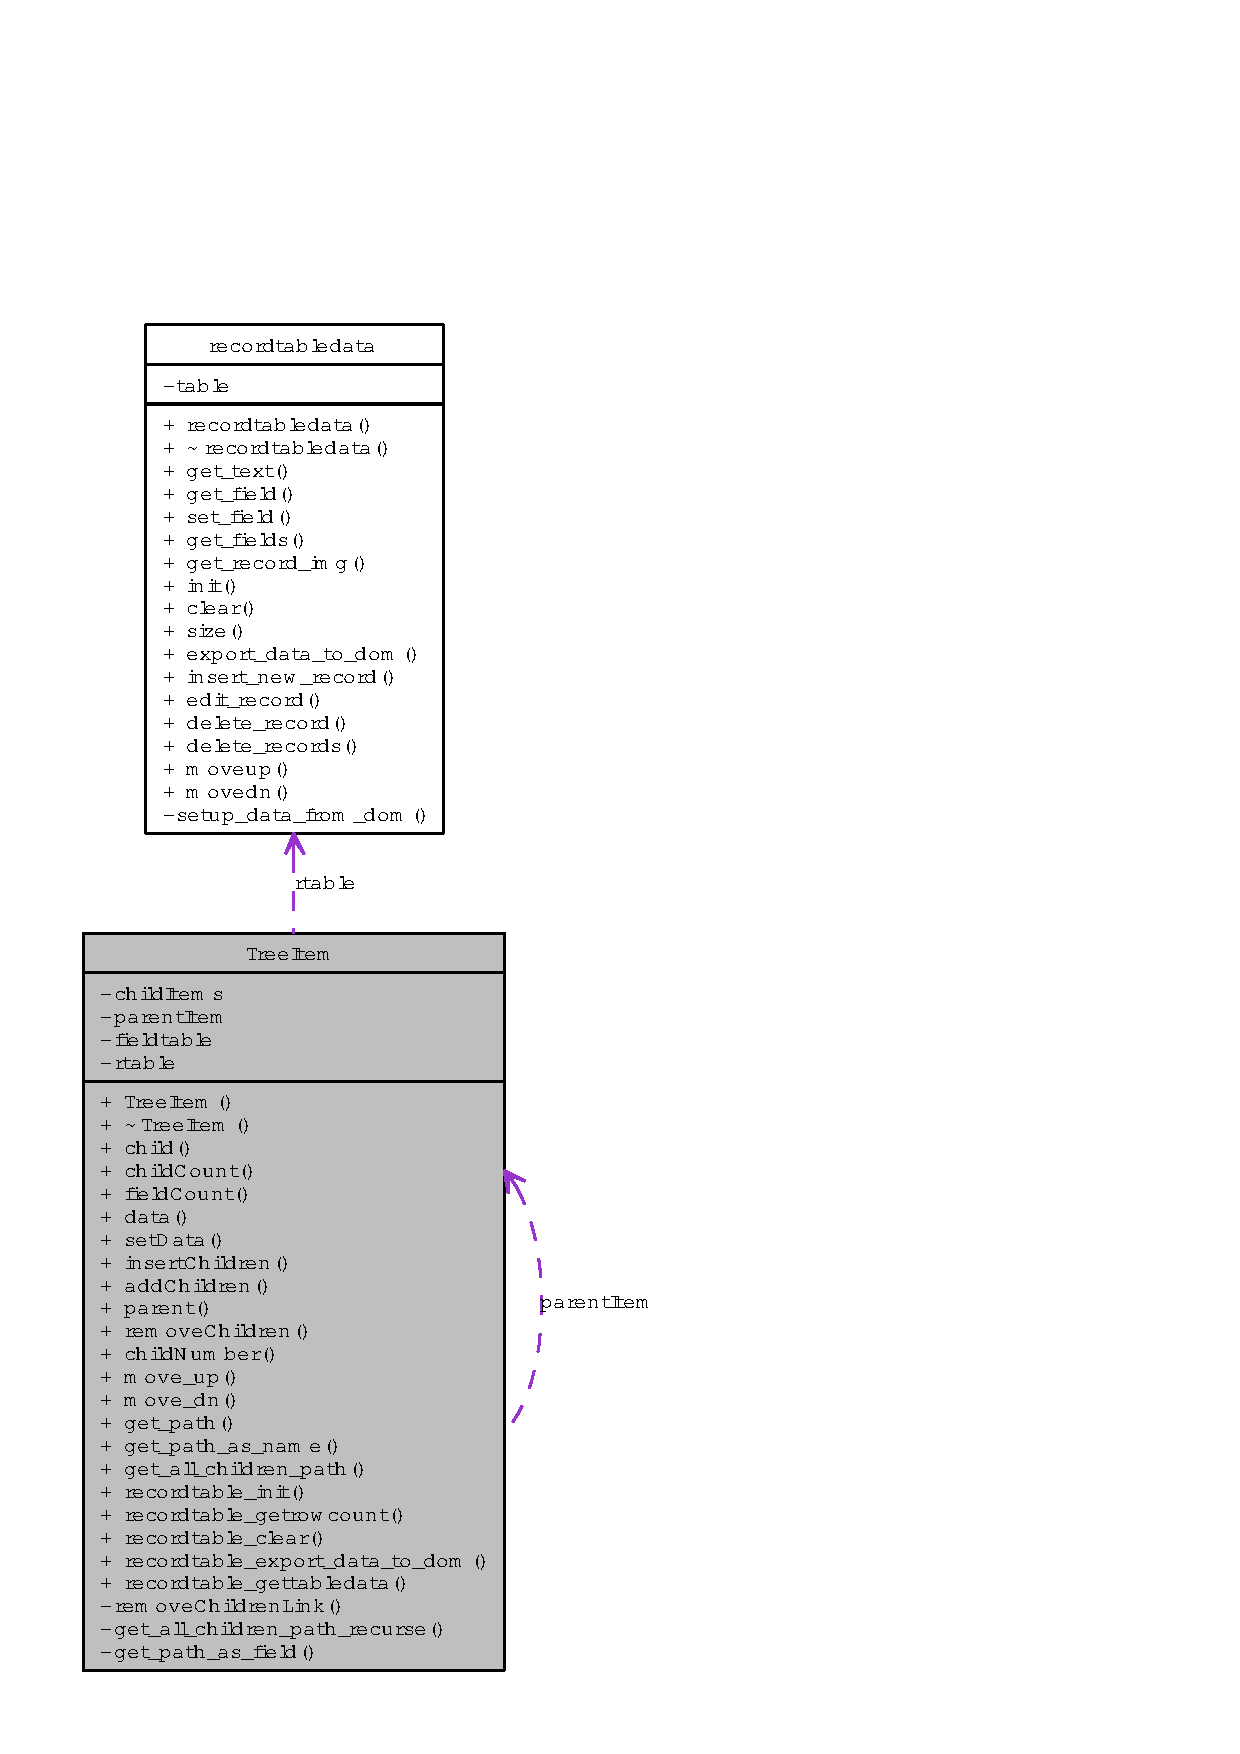
\includegraphics[width=160pt]{classTreeItem__coll__graph}
\end{center}
\end{figure}
\subsection*{Public Member Functions}
\begin{CompactItemize}
\item 
{\bf Tree\-Item} (const QMap$<$ QString, QString $>$ \&data, {\bf Tree\-Item} $\ast$parent=0)
\item 
{\bf $\sim$Tree\-Item} ()
\item 
{\bf Tree\-Item} $\ast$ {\bf child} (int number)
\item 
int {\bf child\-Count} () const
\item 
int {\bf field\-Count} () const
\item 
QVariant {\bf data} (QString name)
\item 
void {\bf set\-Data} (QString n, QString v)
\item 
bool {\bf insert\-Children} (int position, int count, int columns)
\item 
bool {\bf add\-Children} (void)
\item 
{\bf Tree\-Item} $\ast$ {\bf parent} ()
\item 
bool {\bf remove\-Children} (int position, int count)
\item 
int {\bf child\-Number} () const
\item 
bool {\bf move\_\-up} (void)
\item 
bool {\bf move\_\-dn} (void)
\item 
QString\-List {\bf get\_\-path} (void)
\item 
QString\-List {\bf get\_\-path\_\-as\_\-name} (void)
\item 
QList$<$ QString\-List $>$ {\bf get\_\-all\_\-children\_\-path} (void)
\item 
void {\bf recordtable\_\-init} (QDom\-Element dommodel)
\item 
int {\bf recordtable\_\-getrowcount} (void)
\item 
void {\bf recordtable\_\-clear} (void)
\item 
QDom\-Document {\bf recordtable\_\-export\_\-data\_\-to\_\-dom} (void)
\item 
{\bf recordtabledata} $\ast$ {\bf recordtable\_\-gettabledata} (void)
\end{CompactItemize}
\subsection*{Private Member Functions}
\begin{CompactItemize}
\item 
bool {\bf remove\-Children\-Link} (int position, int count)
\item 
QList$<$ QString\-List $>$ {\bf get\_\-all\_\-children\_\-path\_\-recurse} ({\bf Tree\-Item} $\ast$item, int mode)
\item 
QString\-List {\bf get\_\-path\_\-as\_\-field} (QString field)
\end{CompactItemize}
\subsection*{Private Attributes}
\begin{CompactItemize}
\item 
QList$<$ {\bf Tree\-Item} $\ast$ $>$ {\bf child\-Items}
\item 
{\bf Tree\-Item} $\ast$ {\bf parent\-Item}
\item 
QMap$<$ QString, QString $>$ {\bf fieldtable}
\item 
{\bf recordtabledata} {\bf rtable}
\end{CompactItemize}


\subsection{Detailed Description}




Definition at line 13 of file treeitem.h.

\subsection{Constructor \& Destructor Documentation}
\index{TreeItem@{Tree\-Item}!TreeItem@{TreeItem}}
\index{TreeItem@{TreeItem}!TreeItem@{Tree\-Item}}
\subsubsection{\setlength{\rightskip}{0pt plus 5cm}Tree\-Item::Tree\-Item (const QMap$<$ QString, QString $>$ \& {\em data}, {\bf Tree\-Item} $\ast$ {\em parent} = {\tt 0})}\label{classTreeItem_508184fa6523340f5456e530e492e2a4}




Definition at line 13 of file treeitem.cpp.

References fieldtable, parent(), and parent\-Item.

Referenced by add\-Children(), and insert\-Children().

Here is the call graph for this function:\begin{figure}[H]
\begin{center}
\leavevmode
\includegraphics[width=147pt]{classTreeItem_508184fa6523340f5456e530e492e2a4_cgraph}
\end{center}
\end{figure}


Here is the caller graph for this function:\begin{figure}[H]
\begin{center}
\leavevmode
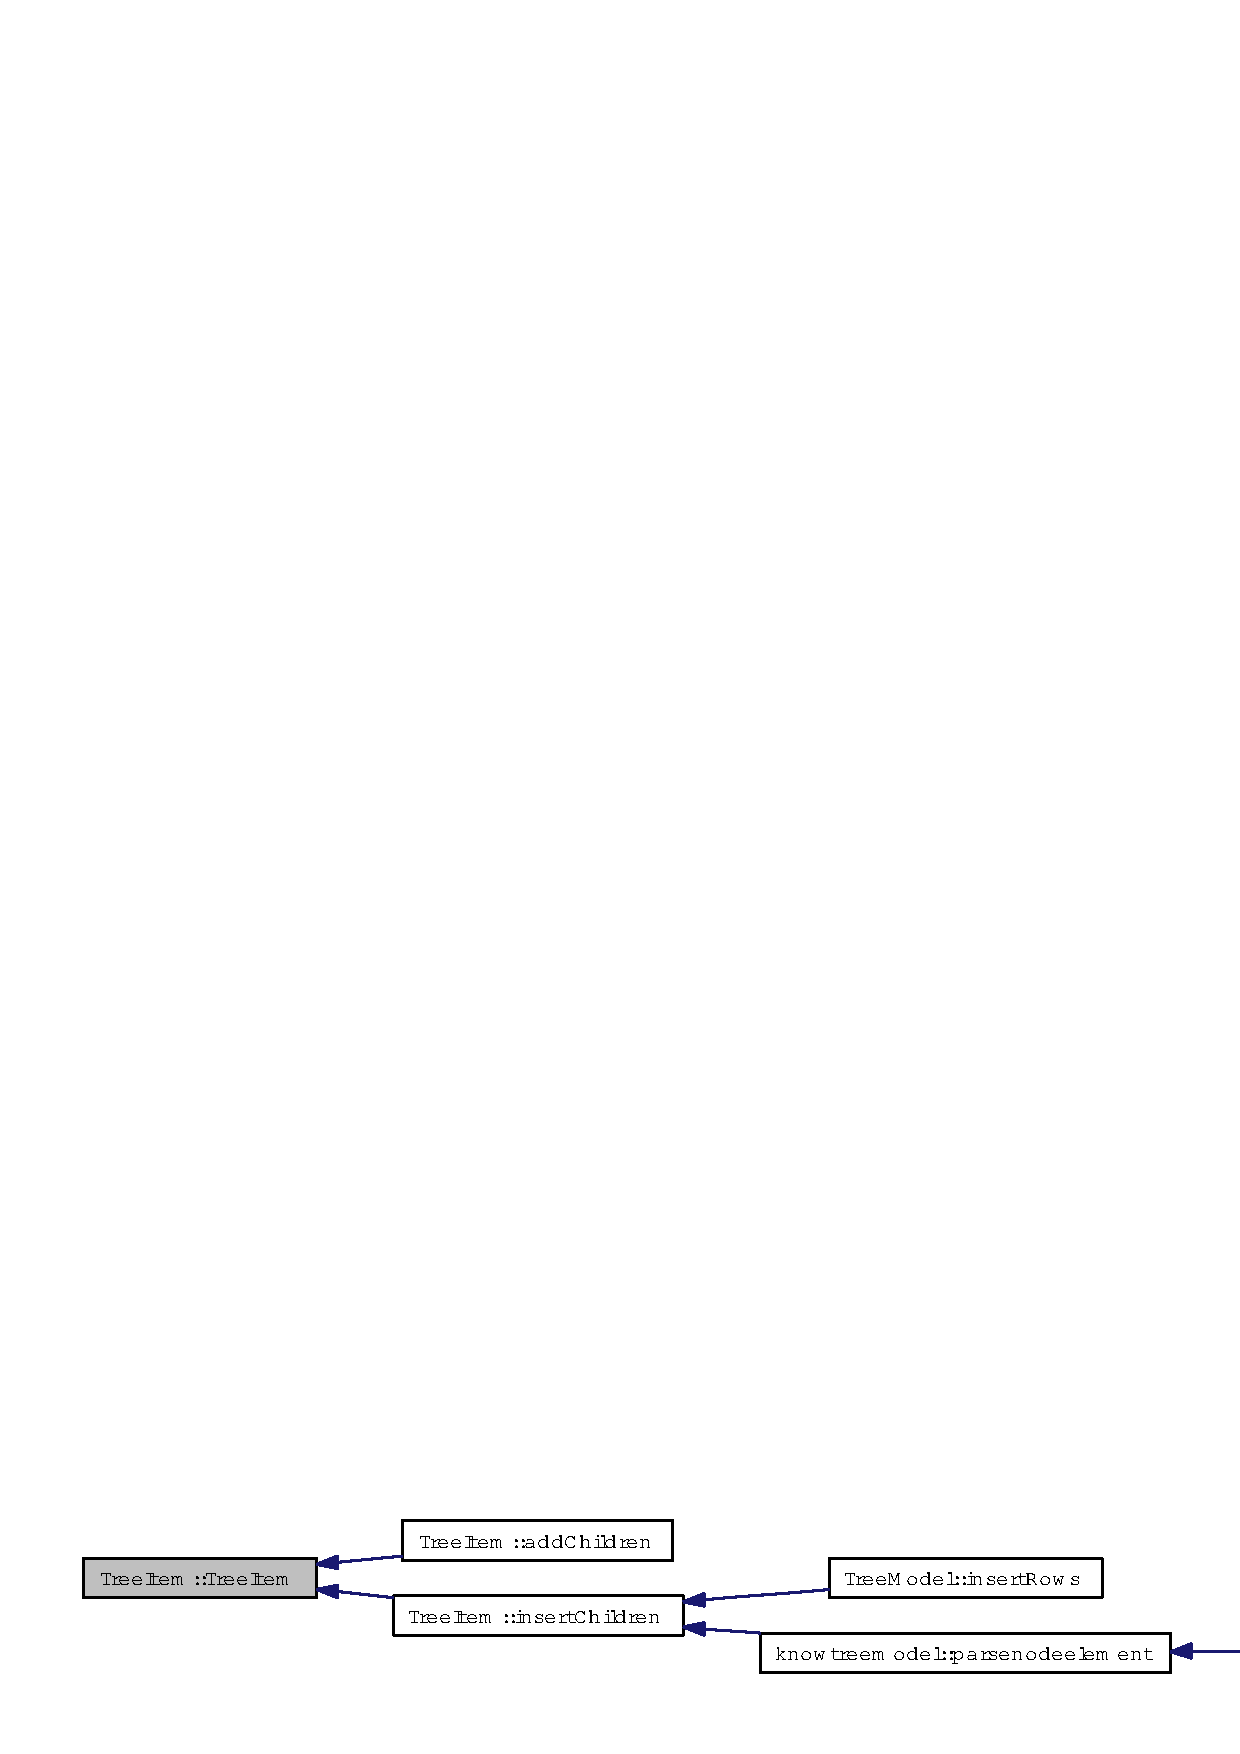
\includegraphics[width=394pt]{classTreeItem_508184fa6523340f5456e530e492e2a4_icgraph}
\end{center}
\end{figure}
\index{TreeItem@{Tree\-Item}!~TreeItem@{$\sim$TreeItem}}
\index{~TreeItem@{$\sim$TreeItem}!TreeItem@{Tree\-Item}}
\subsubsection{\setlength{\rightskip}{0pt plus 5cm}Tree\-Item::$\sim$Tree\-Item ()}\label{classTreeItem_859429185d908c3e54861bbbfb185425}




Definition at line 20 of file treeitem.cpp.

References child\-Items, and recordtable\_\-clear().

Here is the call graph for this function:\begin{figure}[H]
\begin{center}
\leavevmode
\includegraphics[width=369pt]{classTreeItem_859429185d908c3e54861bbbfb185425_cgraph}
\end{center}
\end{figure}


\subsection{Member Function Documentation}
\index{TreeItem@{Tree\-Item}!child@{child}}
\index{child@{child}!TreeItem@{Tree\-Item}}
\subsubsection{\setlength{\rightskip}{0pt plus 5cm}{\bf Tree\-Item} $\ast$ Tree\-Item::child (int {\em number})}\label{classTreeItem_993f98a911be40cc1466e105b4657bbe}




Definition at line 34 of file treeitem.cpp.

References child\-Items.

Referenced by findscreen::find\_\-recurse(), get\_\-all\_\-children\_\-path\_\-recurse(), Tree\-Model::get\-Item(), Tree\-Model::index(), knowtreemodel::index\-Children(), knowtreemodel::parsenodeelement(), and knowtreemodel::parsetreetodom().

Here is the caller graph for this function:\begin{figure}[H]
\begin{center}
\leavevmode
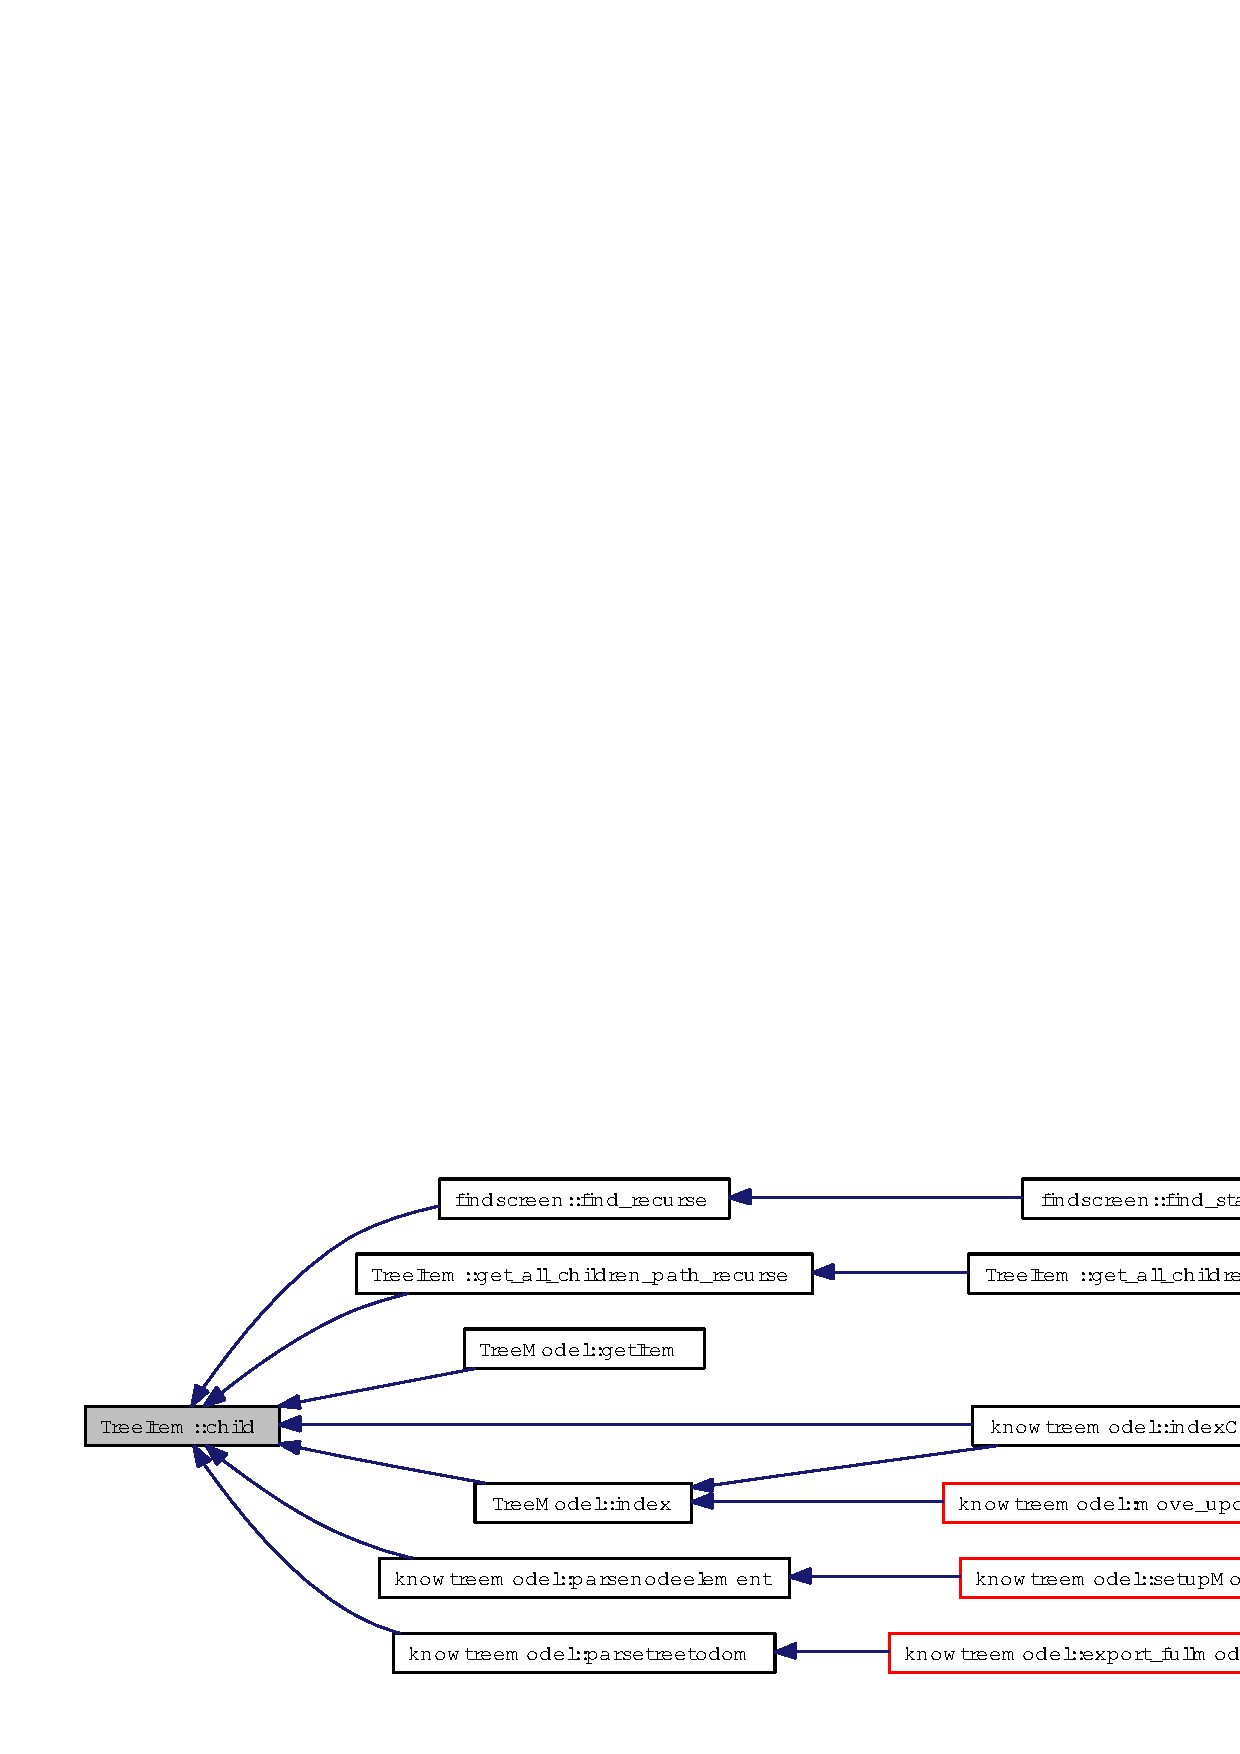
\includegraphics[width=342pt]{classTreeItem_993f98a911be40cc1466e105b4657bbe_icgraph}
\end{center}
\end{figure}
\index{TreeItem@{Tree\-Item}!childCount@{childCount}}
\index{childCount@{childCount}!TreeItem@{Tree\-Item}}
\subsubsection{\setlength{\rightskip}{0pt plus 5cm}int Tree\-Item::child\-Count () const}\label{classTreeItem_14551ec37f50067974fc93aa78b4b6e1}




Definition at line 41 of file treeitem.cpp.

References child\-Items.

Referenced by findscreen::find\_\-recurse(), get\_\-all\_\-children\_\-path\_\-recurse(), Tree\-Model::get\-Item(), knowtreemodel::index\-Children(), treescreen::ins\_\-branch(), treescreen::ins\_\-subbranch(), move\_\-dn(), knowtreemodel::parsenodeelement(), knowtreemodel::parsetreetodom(), and Tree\-Model::row\-Count().

Here is the caller graph for this function:\begin{figure}[H]
\begin{center}
\leavevmode
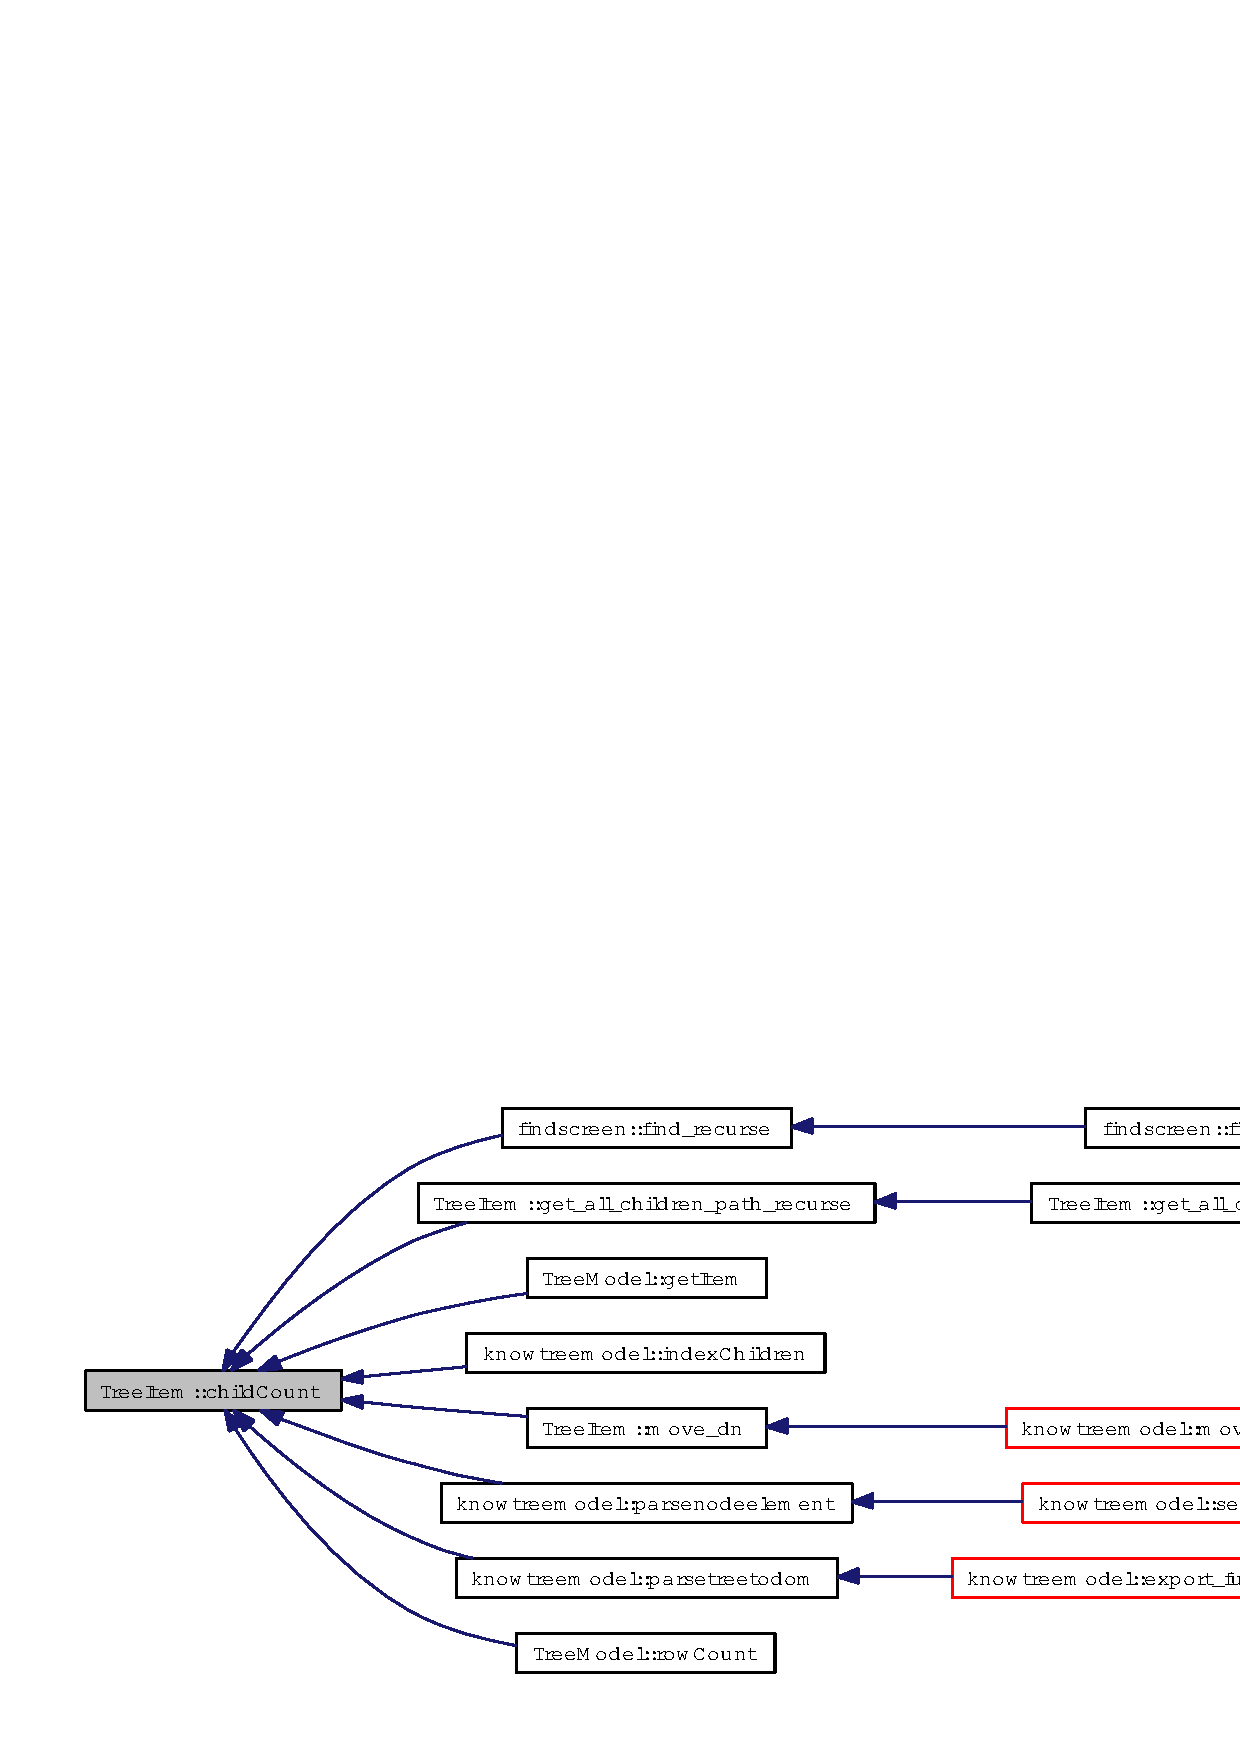
\includegraphics[width=357pt]{classTreeItem_14551ec37f50067974fc93aa78b4b6e1_icgraph}
\end{center}
\end{figure}
\index{TreeItem@{Tree\-Item}!fieldCount@{fieldCount}}
\index{fieldCount@{fieldCount}!TreeItem@{Tree\-Item}}
\subsubsection{\setlength{\rightskip}{0pt plus 5cm}int Tree\-Item::field\-Count () const}\label{classTreeItem_d2c76cd733694499499c0b2e423756f5}




Definition at line 58 of file treeitem.cpp.

References fieldtable.\index{TreeItem@{Tree\-Item}!data@{data}}
\index{data@{data}!TreeItem@{Tree\-Item}}
\subsubsection{\setlength{\rightskip}{0pt plus 5cm}QVariant Tree\-Item::data (QString {\em name})}\label{classTreeItem_30f59edac140c6fa48b5f09315e15a65}




Definition at line 65 of file treeitem.cpp.

References critical\_\-error(), fieldtable, and recordtable\_\-getrowcount().

Referenced by add\-Children(), Tree\-Model::data(), treescreen::del\_\-branch(), treescreen::edit\_\-branch(), findscreen::find\_\-recurse(), get\_\-path\_\-as\_\-field(), insert\-Children(), knowtreemodel::parsetreetodom(), and mainwindow::set\_\-tree\_\-position().

Here is the call graph for this function:\begin{figure}[H]
\begin{center}
\leavevmode
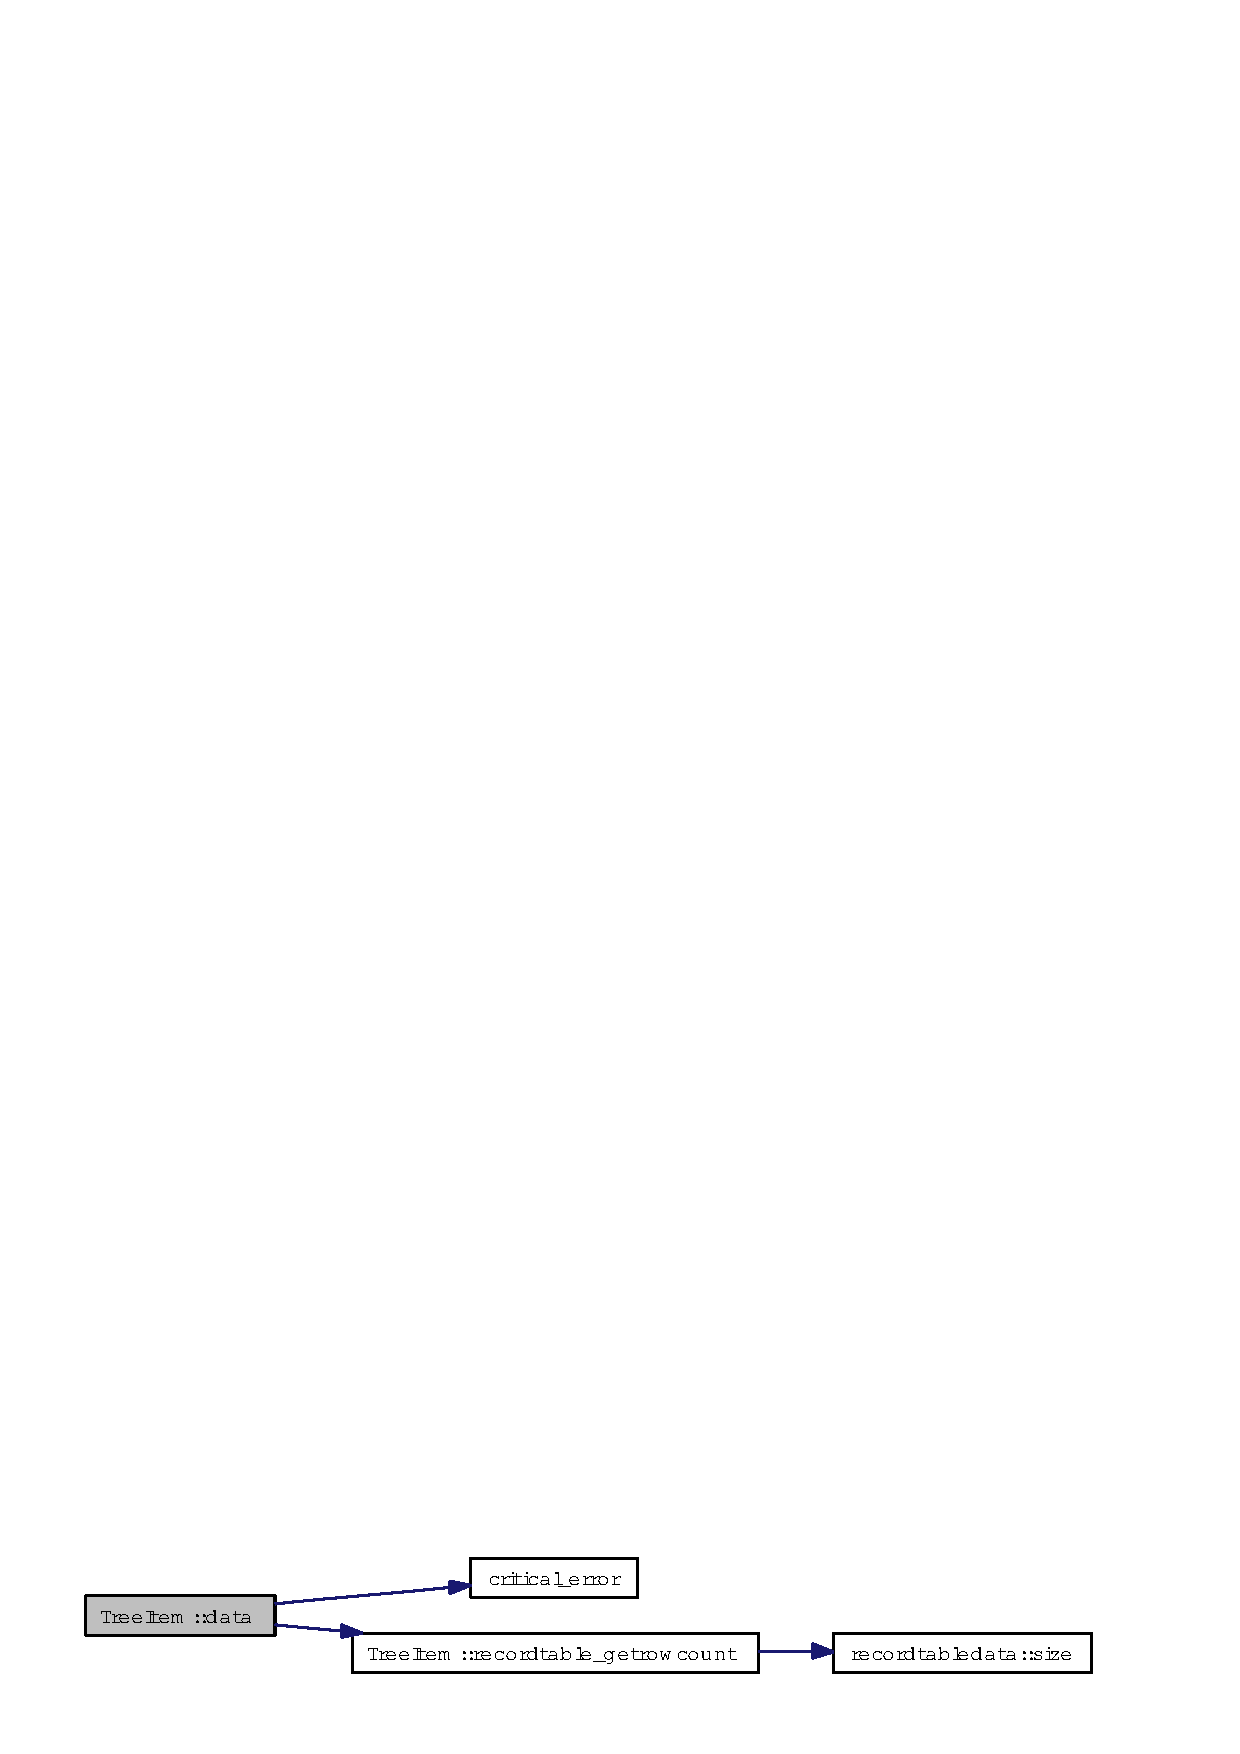
\includegraphics[width=264pt]{classTreeItem_30f59edac140c6fa48b5f09315e15a65_cgraph}
\end{center}
\end{figure}


Here is the caller graph for this function:\begin{figure}[H]
\begin{center}
\leavevmode
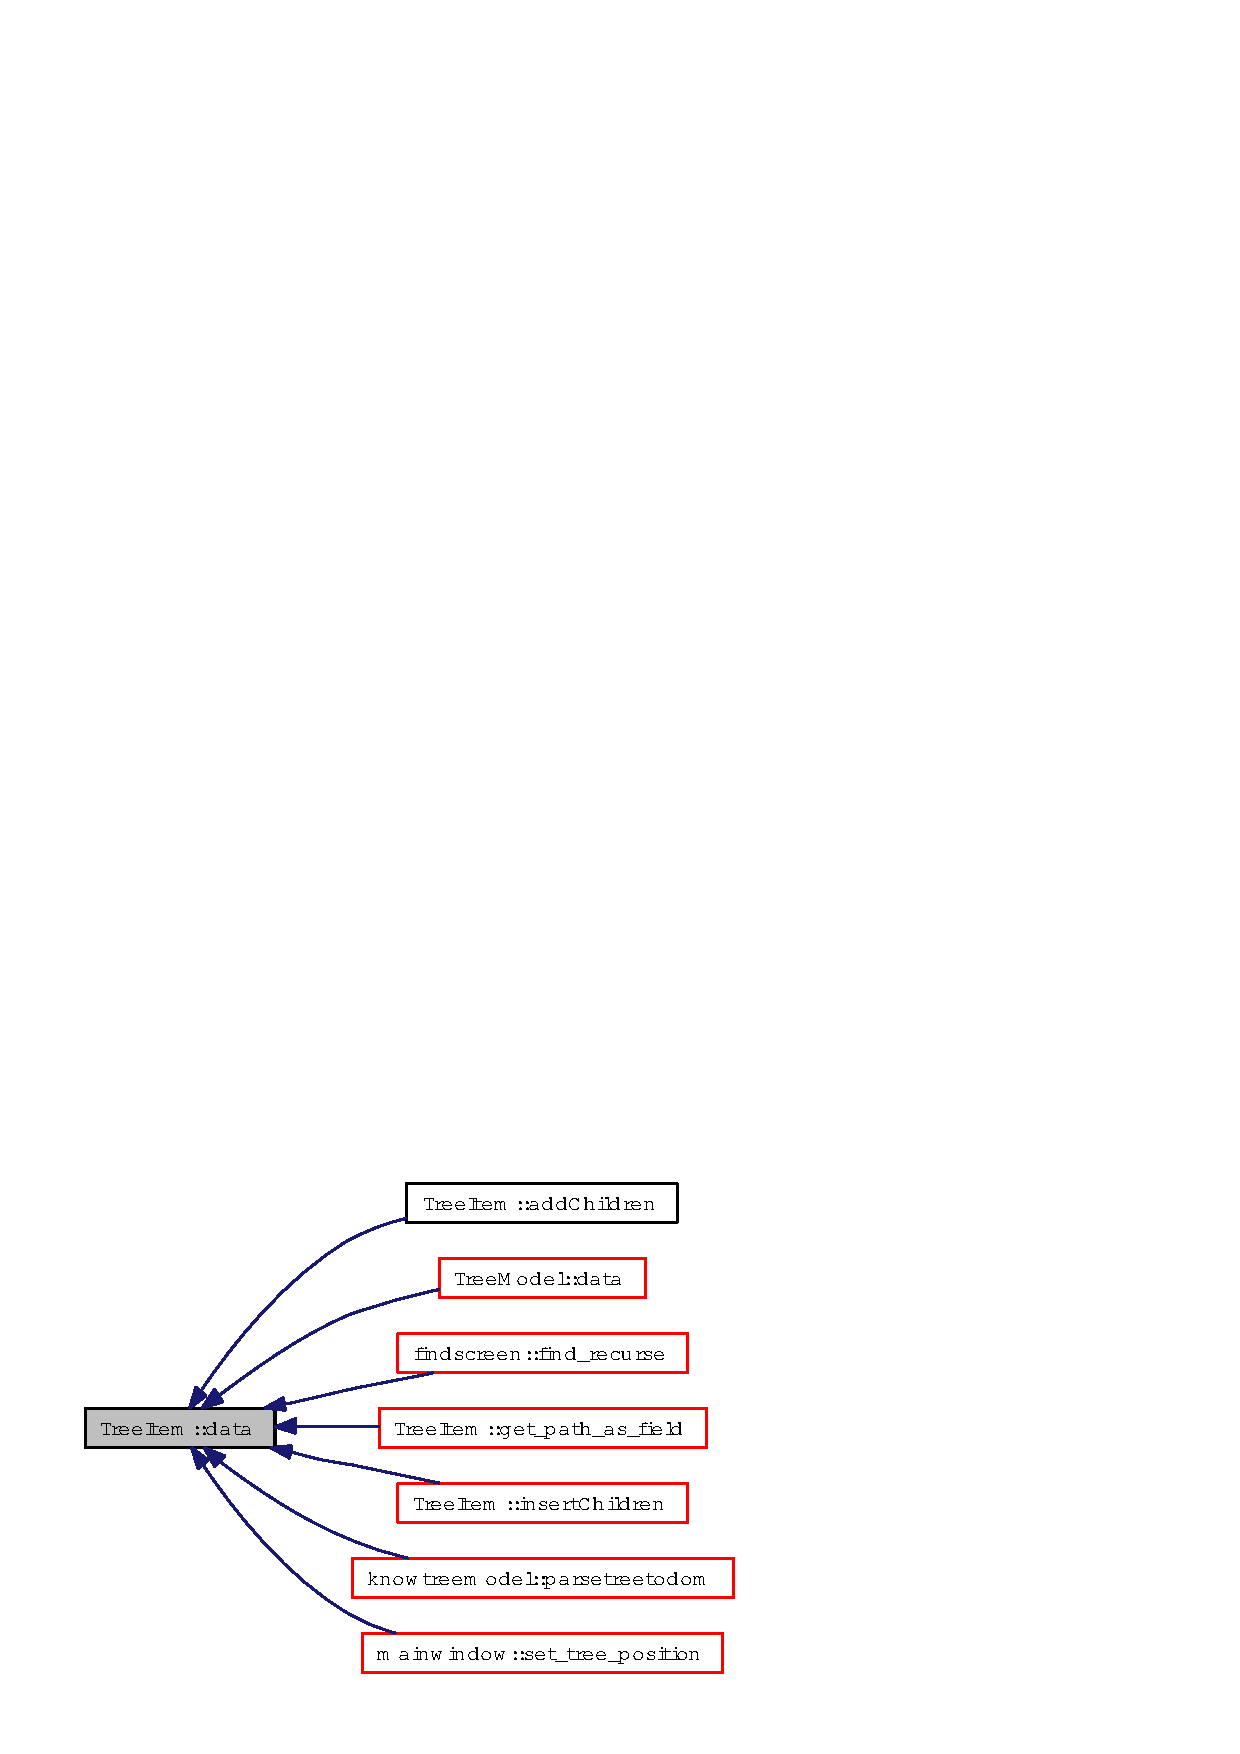
\includegraphics[width=178pt]{classTreeItem_30f59edac140c6fa48b5f09315e15a65_icgraph}
\end{center}
\end{figure}
\index{TreeItem@{Tree\-Item}!setData@{setData}}
\index{setData@{setData}!TreeItem@{Tree\-Item}}
\subsubsection{\setlength{\rightskip}{0pt plus 5cm}void Tree\-Item::set\-Data (QString {\em n}, QString {\em v})}\label{classTreeItem_4e613f935d91a595e2b61e06726bc364}




Definition at line 101 of file treeitem.cpp.

References fieldtable.

Referenced by treescreen::edit\_\-branch(), Tree\-Model::set\-Data(), and Tree\-Model::set\-Header\-Data().

Here is the caller graph for this function:\begin{figure}[H]
\begin{center}
\leavevmode
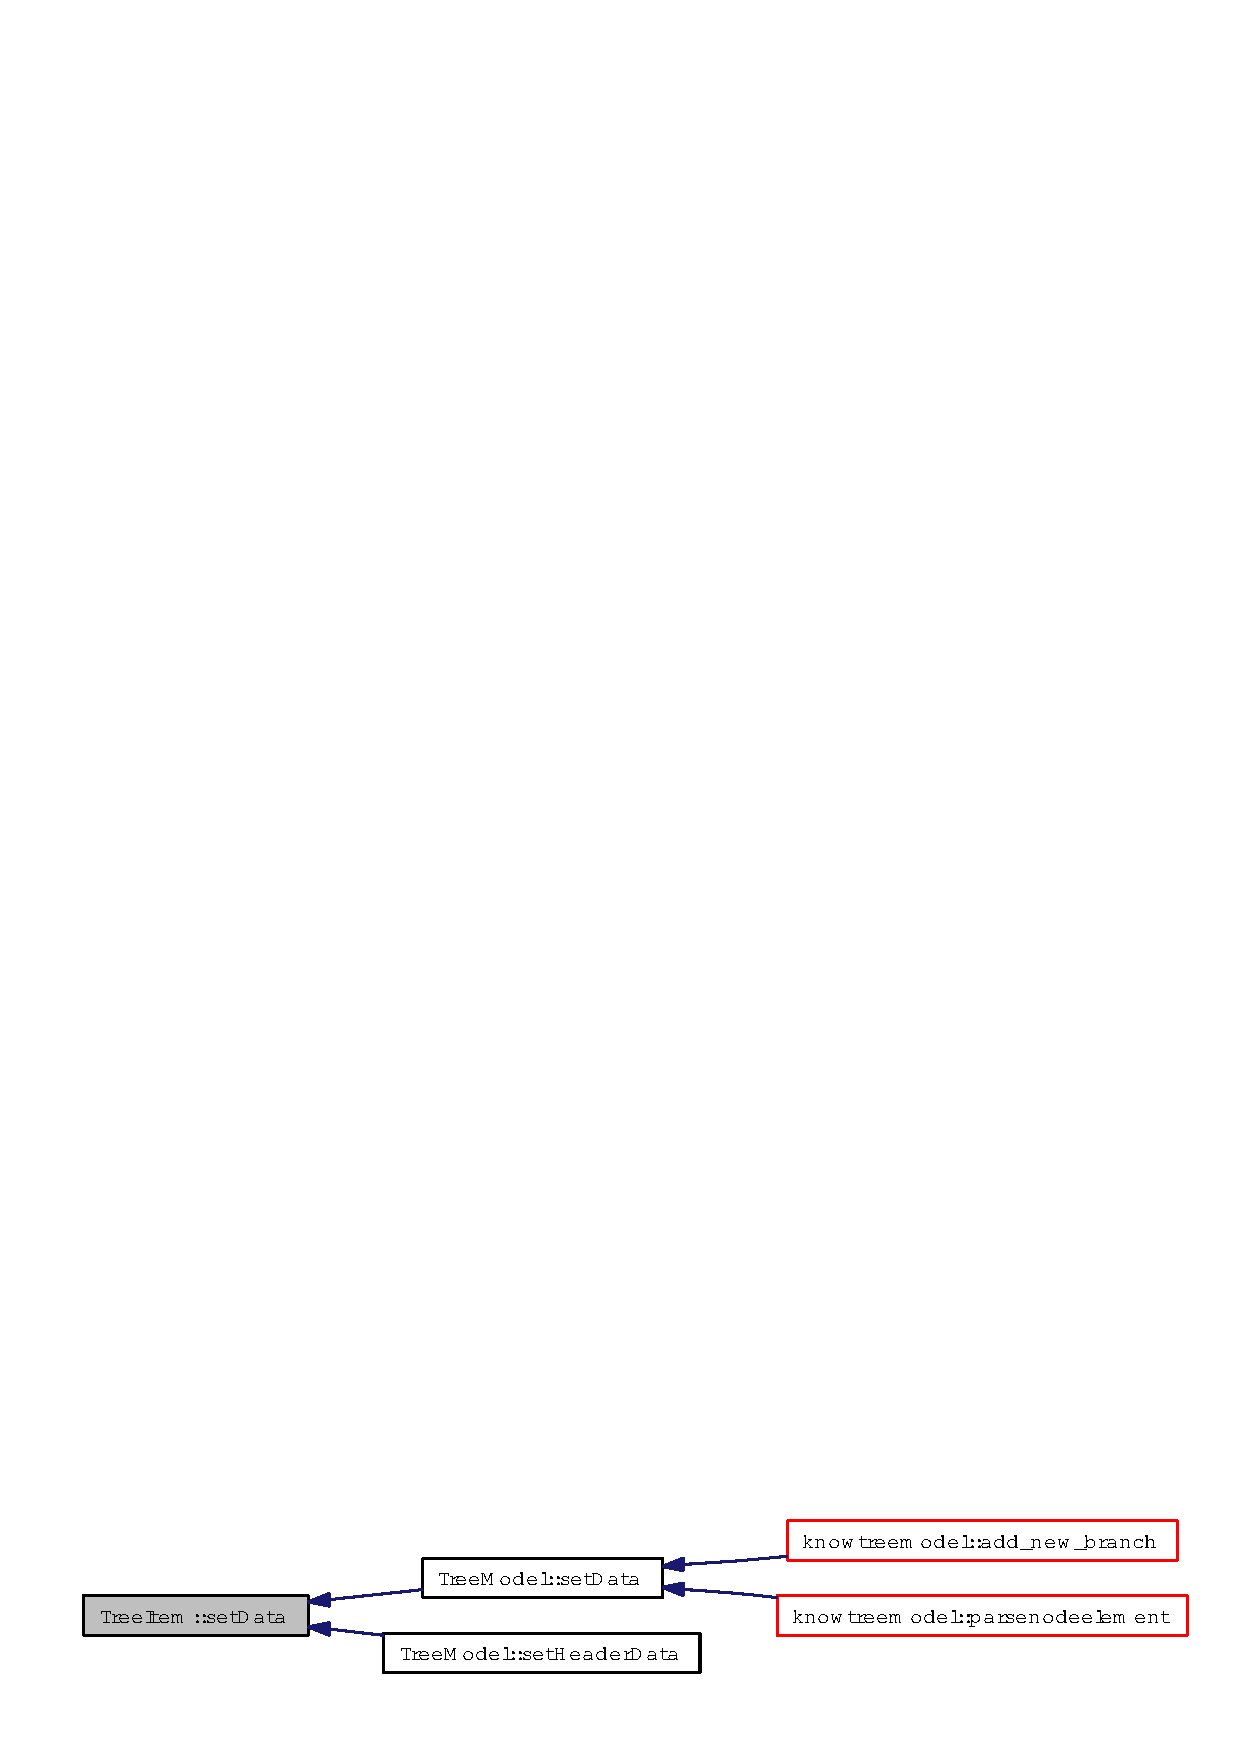
\includegraphics[width=287pt]{classTreeItem_4e613f935d91a595e2b61e06726bc364_icgraph}
\end{center}
\end{figure}
\index{TreeItem@{Tree\-Item}!insertChildren@{insertChildren}}
\index{insertChildren@{insertChildren}!TreeItem@{Tree\-Item}}
\subsubsection{\setlength{\rightskip}{0pt plus 5cm}bool Tree\-Item::insert\-Children (int {\em position}, int {\em count}, int {\em columns})}\label{classTreeItem_d6b6da67cc03e79c714419f93f5005c6}




Definition at line 128 of file treeitem.cpp.

References child\-Items, data(), and Tree\-Item().

Referenced by Tree\-Model::insert\-Rows(), and knowtreemodel::parsenodeelement().

Here is the call graph for this function:\begin{figure}[H]
\begin{center}
\leavevmode
\includegraphics[width=362pt]{classTreeItem_d6b6da67cc03e79c714419f93f5005c6_cgraph}
\end{center}
\end{figure}


Here is the caller graph for this function:\begin{figure}[H]
\begin{center}
\leavevmode
\includegraphics[width=320pt]{classTreeItem_d6b6da67cc03e79c714419f93f5005c6_icgraph}
\end{center}
\end{figure}
\index{TreeItem@{Tree\-Item}!addChildren@{addChildren}}
\index{addChildren@{addChildren}!TreeItem@{Tree\-Item}}
\subsubsection{\setlength{\rightskip}{0pt plus 5cm}bool Tree\-Item::add\-Children (void)}\label{classTreeItem_fcb572391879aa48a2ca55b43b4d987d}




Definition at line 145 of file treeitem.cpp.

References child\-Items, data(), and Tree\-Item().

Here is the call graph for this function:\begin{figure}[H]
\begin{center}
\leavevmode
\includegraphics[width=357pt]{classTreeItem_fcb572391879aa48a2ca55b43b4d987d_cgraph}
\end{center}
\end{figure}
\index{TreeItem@{Tree\-Item}!parent@{parent}}
\index{parent@{parent}!TreeItem@{Tree\-Item}}
\subsubsection{\setlength{\rightskip}{0pt plus 5cm}{\bf Tree\-Item} $\ast$ Tree\-Item::parent ()}\label{classTreeItem_392ec493dfab91ee474d7ff83e2c0211}




Definition at line 118 of file treeitem.cpp.

References parent\-Item.

Referenced by knowtreemodel::add\_\-new\_\-sibling\_\-branch(), get\_\-path\_\-as\_\-field(), treescreen::ins\_\-branch(), Tree\-Model::parent(), and Tree\-Item().

Here is the caller graph for this function:\begin{figure}[H]
\begin{center}
\leavevmode
\includegraphics[width=301pt]{classTreeItem_392ec493dfab91ee474d7ff83e2c0211_icgraph}
\end{center}
\end{figure}
\index{TreeItem@{Tree\-Item}!removeChildren@{removeChildren}}
\index{removeChildren@{removeChildren}!TreeItem@{Tree\-Item}}
\subsubsection{\setlength{\rightskip}{0pt plus 5cm}bool Tree\-Item::remove\-Children (int {\em position}, int {\em count})}\label{classTreeItem_a9861c44a34b210bde61527b9b5018f3}




Definition at line 157 of file treeitem.cpp.

References child\-Items.

Referenced by Tree\-Model::remove\-Rows().

Here is the caller graph for this function:\begin{figure}[H]
\begin{center}
\leavevmode
\includegraphics[width=186pt]{classTreeItem_a9861c44a34b210bde61527b9b5018f3_icgraph}
\end{center}
\end{figure}
\index{TreeItem@{Tree\-Item}!childNumber@{childNumber}}
\index{childNumber@{childNumber}!TreeItem@{Tree\-Item}}
\subsubsection{\setlength{\rightskip}{0pt plus 5cm}int Tree\-Item::child\-Number () const}\label{classTreeItem_87e01b18fd3b575ef1338545380228f5}




Definition at line 49 of file treeitem.cpp.

References child\-Items, and parent\-Item.

Referenced by knowtreemodel::get\_\-item\_\-index(), move\_\-dn(), move\_\-up(), and Tree\-Model::parent().

Here is the caller graph for this function:\begin{figure}[H]
\begin{center}
\leavevmode
\includegraphics[width=197pt]{classTreeItem_87e01b18fd3b575ef1338545380228f5_icgraph}
\end{center}
\end{figure}
\index{TreeItem@{Tree\-Item}!move_up@{move\_\-up}}
\index{move_up@{move\_\-up}!TreeItem@{Tree\-Item}}
\subsubsection{\setlength{\rightskip}{0pt plus 5cm}bool Tree\-Item::move\_\-up (void)}\label{classTreeItem_207f6579c483068f8d2da4b1302705fc}




Definition at line 182 of file treeitem.cpp.

References child\-Items, child\-Number(), and parent\-Item.

Referenced by knowtreemodel::move\_\-updn\_\-branch().

Here is the call graph for this function:\begin{figure}[H]
\begin{center}
\leavevmode
\includegraphics[width=165pt]{classTreeItem_207f6579c483068f8d2da4b1302705fc_cgraph}
\end{center}
\end{figure}


Here is the caller graph for this function:\begin{figure}[H]
\begin{center}
\leavevmode
\includegraphics[width=311pt]{classTreeItem_207f6579c483068f8d2da4b1302705fc_icgraph}
\end{center}
\end{figure}
\index{TreeItem@{Tree\-Item}!move_dn@{move\_\-dn}}
\index{move_dn@{move\_\-dn}!TreeItem@{Tree\-Item}}
\subsubsection{\setlength{\rightskip}{0pt plus 5cm}bool Tree\-Item::move\_\-dn (void)}\label{classTreeItem_e47dfb60f0633c684ddc7a46ceb83d0e}




Definition at line 197 of file treeitem.cpp.

References child\-Count(), child\-Items, child\-Number(), and parent\-Item.

Referenced by knowtreemodel::move\_\-updn\_\-branch().

Here is the call graph for this function:\begin{figure}[H]
\begin{center}
\leavevmode
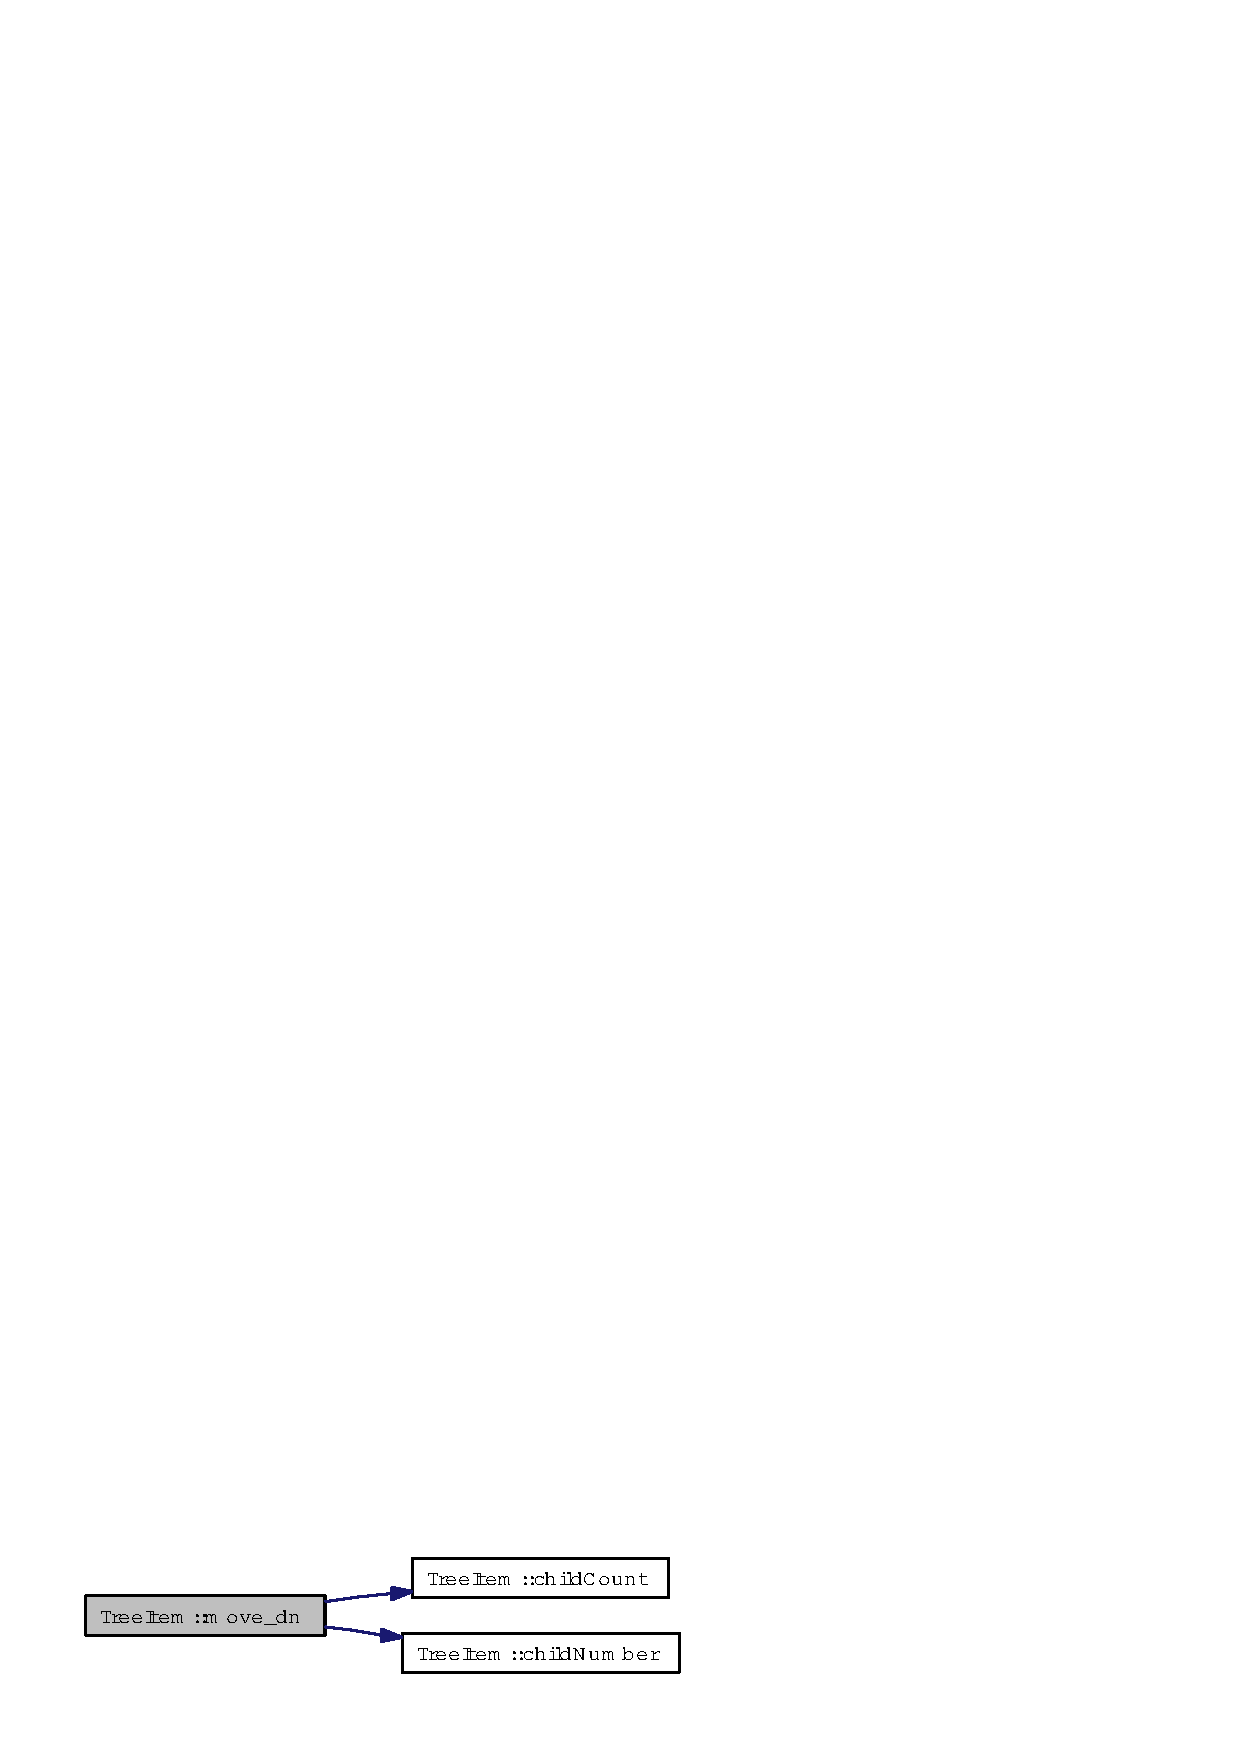
\includegraphics[width=165pt]{classTreeItem_e47dfb60f0633c684ddc7a46ceb83d0e_cgraph}
\end{center}
\end{figure}


Here is the caller graph for this function:\begin{figure}[H]
\begin{center}
\leavevmode
\includegraphics[width=311pt]{classTreeItem_e47dfb60f0633c684ddc7a46ceb83d0e_icgraph}
\end{center}
\end{figure}
\index{TreeItem@{Tree\-Item}!get_path@{get\_\-path}}
\index{get_path@{get\_\-path}!TreeItem@{Tree\-Item}}
\subsubsection{\setlength{\rightskip}{0pt plus 5cm}QString\-List Tree\-Item::get\_\-path (void)}\label{classTreeItem_a47b4b36567db4559ceafc910d70c4da}




Definition at line 213 of file treeitem.cpp.

References get\_\-path\_\-as\_\-field().

Referenced by findscreen::find\_\-recurse(), get\_\-all\_\-children\_\-path\_\-recurse(), and mainwindow::save\_\-tree\_\-position().

Here is the call graph for this function:\begin{figure}[H]
\begin{center}
\leavevmode
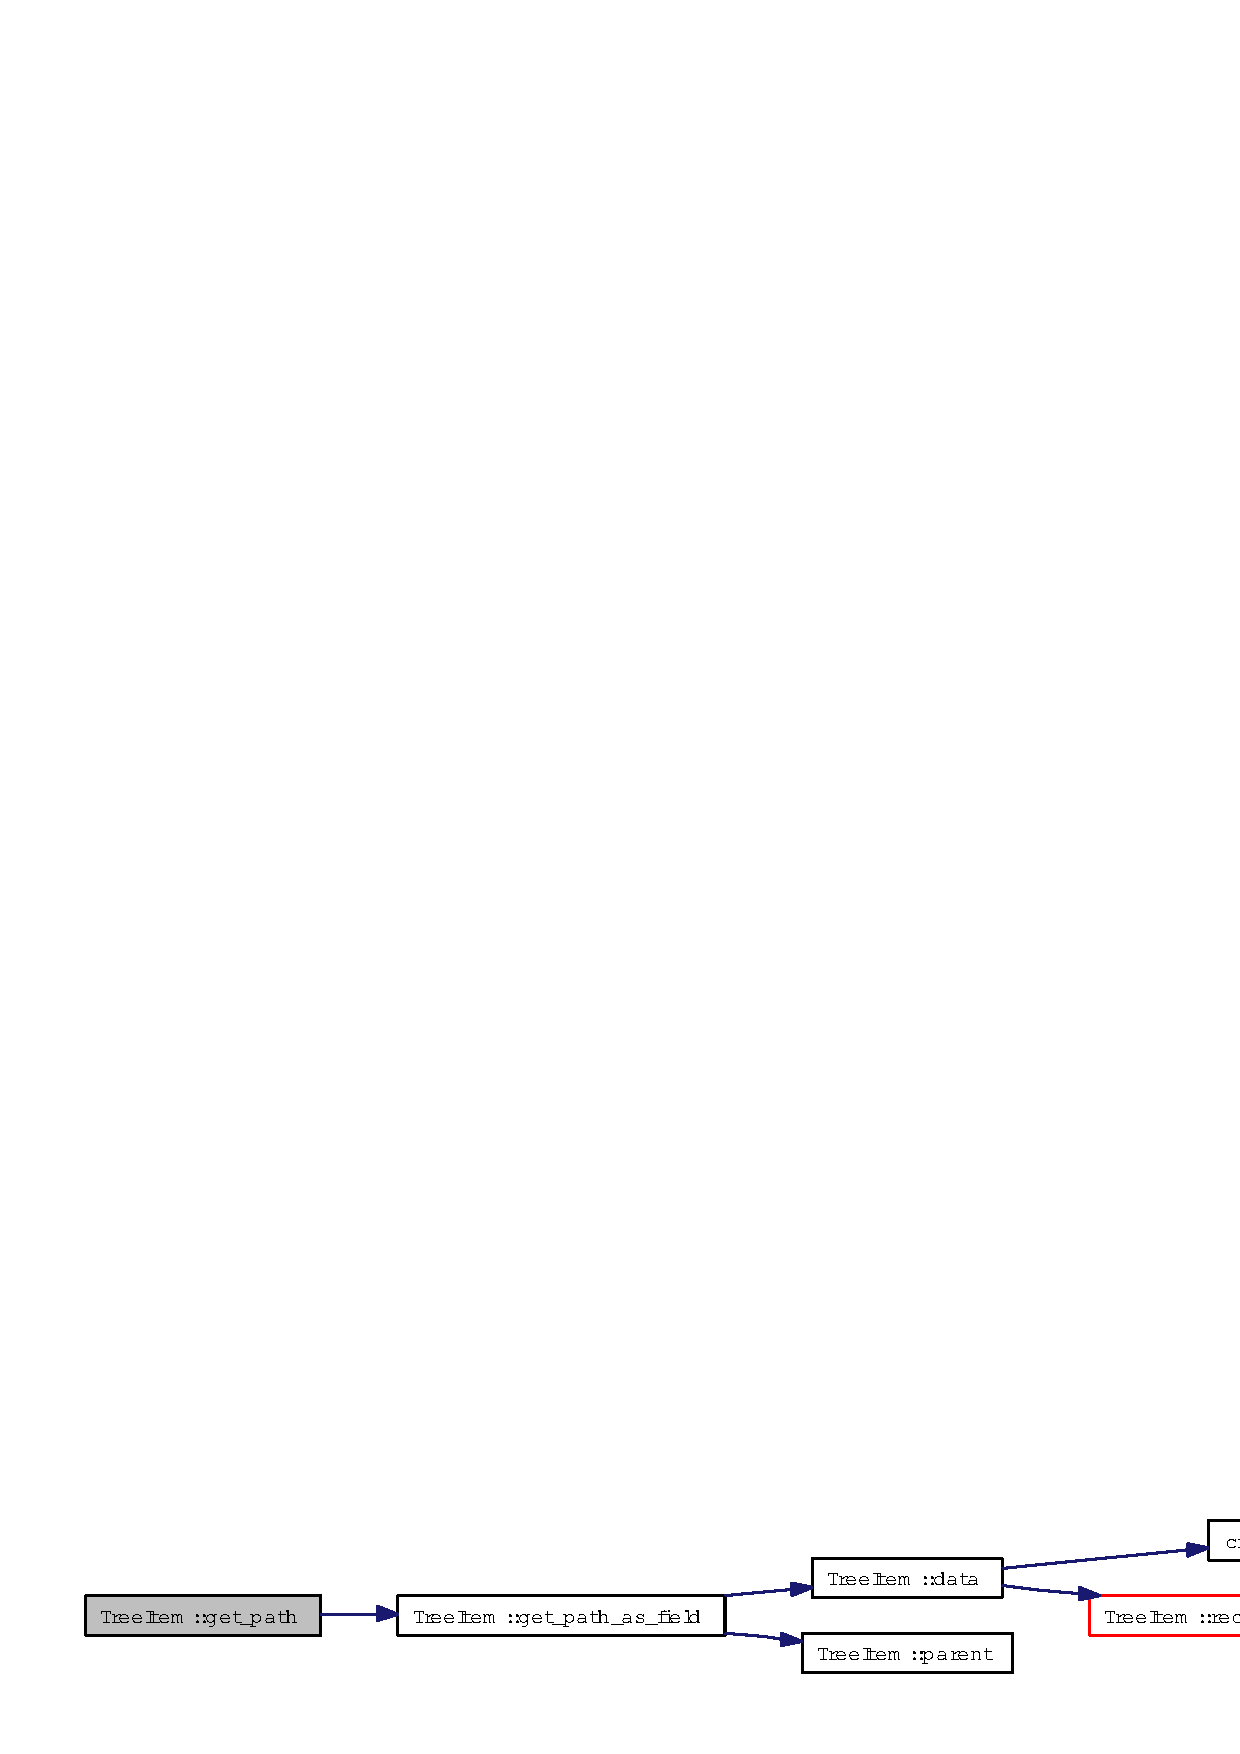
\includegraphics[width=361pt]{classTreeItem_a47b4b36567db4559ceafc910d70c4da_cgraph}
\end{center}
\end{figure}


Here is the caller graph for this function:\begin{figure}[H]
\begin{center}
\leavevmode
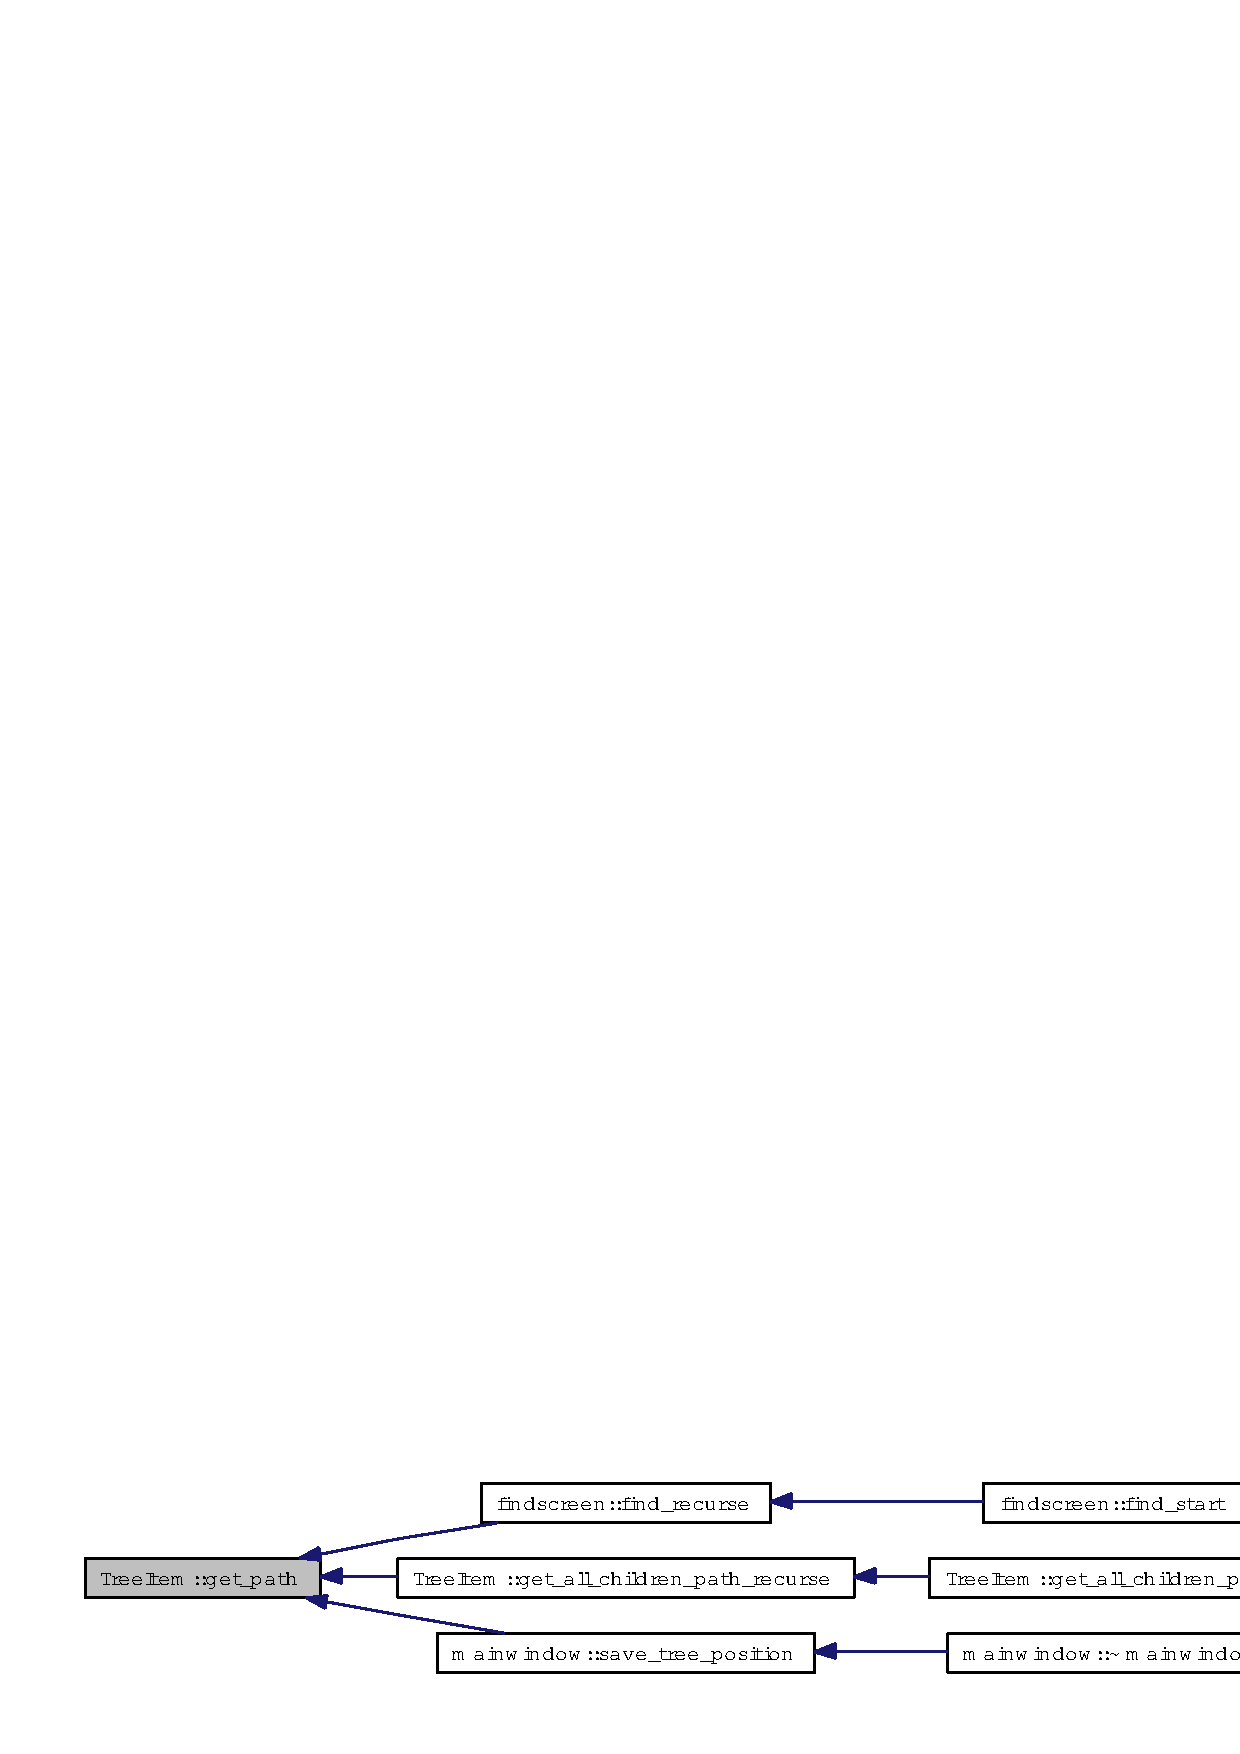
\includegraphics[width=313pt]{classTreeItem_a47b4b36567db4559ceafc910d70c4da_icgraph}
\end{center}
\end{figure}
\index{TreeItem@{Tree\-Item}!get_path_as_name@{get\_\-path\_\-as\_\-name}}
\index{get_path_as_name@{get\_\-path\_\-as\_\-name}!TreeItem@{Tree\-Item}}
\subsubsection{\setlength{\rightskip}{0pt plus 5cm}QString\-List Tree\-Item::get\_\-path\_\-as\_\-name (void)}\label{classTreeItem_9137263215b7354cb66591b7730af9e6}




Definition at line 219 of file treeitem.cpp.

References get\_\-path\_\-as\_\-field().

Here is the call graph for this function:\begin{figure}[H]
\begin{center}
\leavevmode
\includegraphics[width=386pt]{classTreeItem_9137263215b7354cb66591b7730af9e6_cgraph}
\end{center}
\end{figure}
\index{TreeItem@{Tree\-Item}!get_all_children_path@{get\_\-all\_\-children\_\-path}}
\index{get_all_children_path@{get\_\-all\_\-children\_\-path}!TreeItem@{Tree\-Item}}
\subsubsection{\setlength{\rightskip}{0pt plus 5cm}QList$<$ QString\-List $>$ Tree\-Item::get\_\-all\_\-children\_\-path (void)}\label{classTreeItem_cd5987be73e4cd3a16003b6bad3f1e67}




Definition at line 248 of file treeitem.cpp.

References get\_\-all\_\-children\_\-path\_\-recurse().

Here is the call graph for this function:\begin{figure}[H]
\begin{center}
\leavevmode
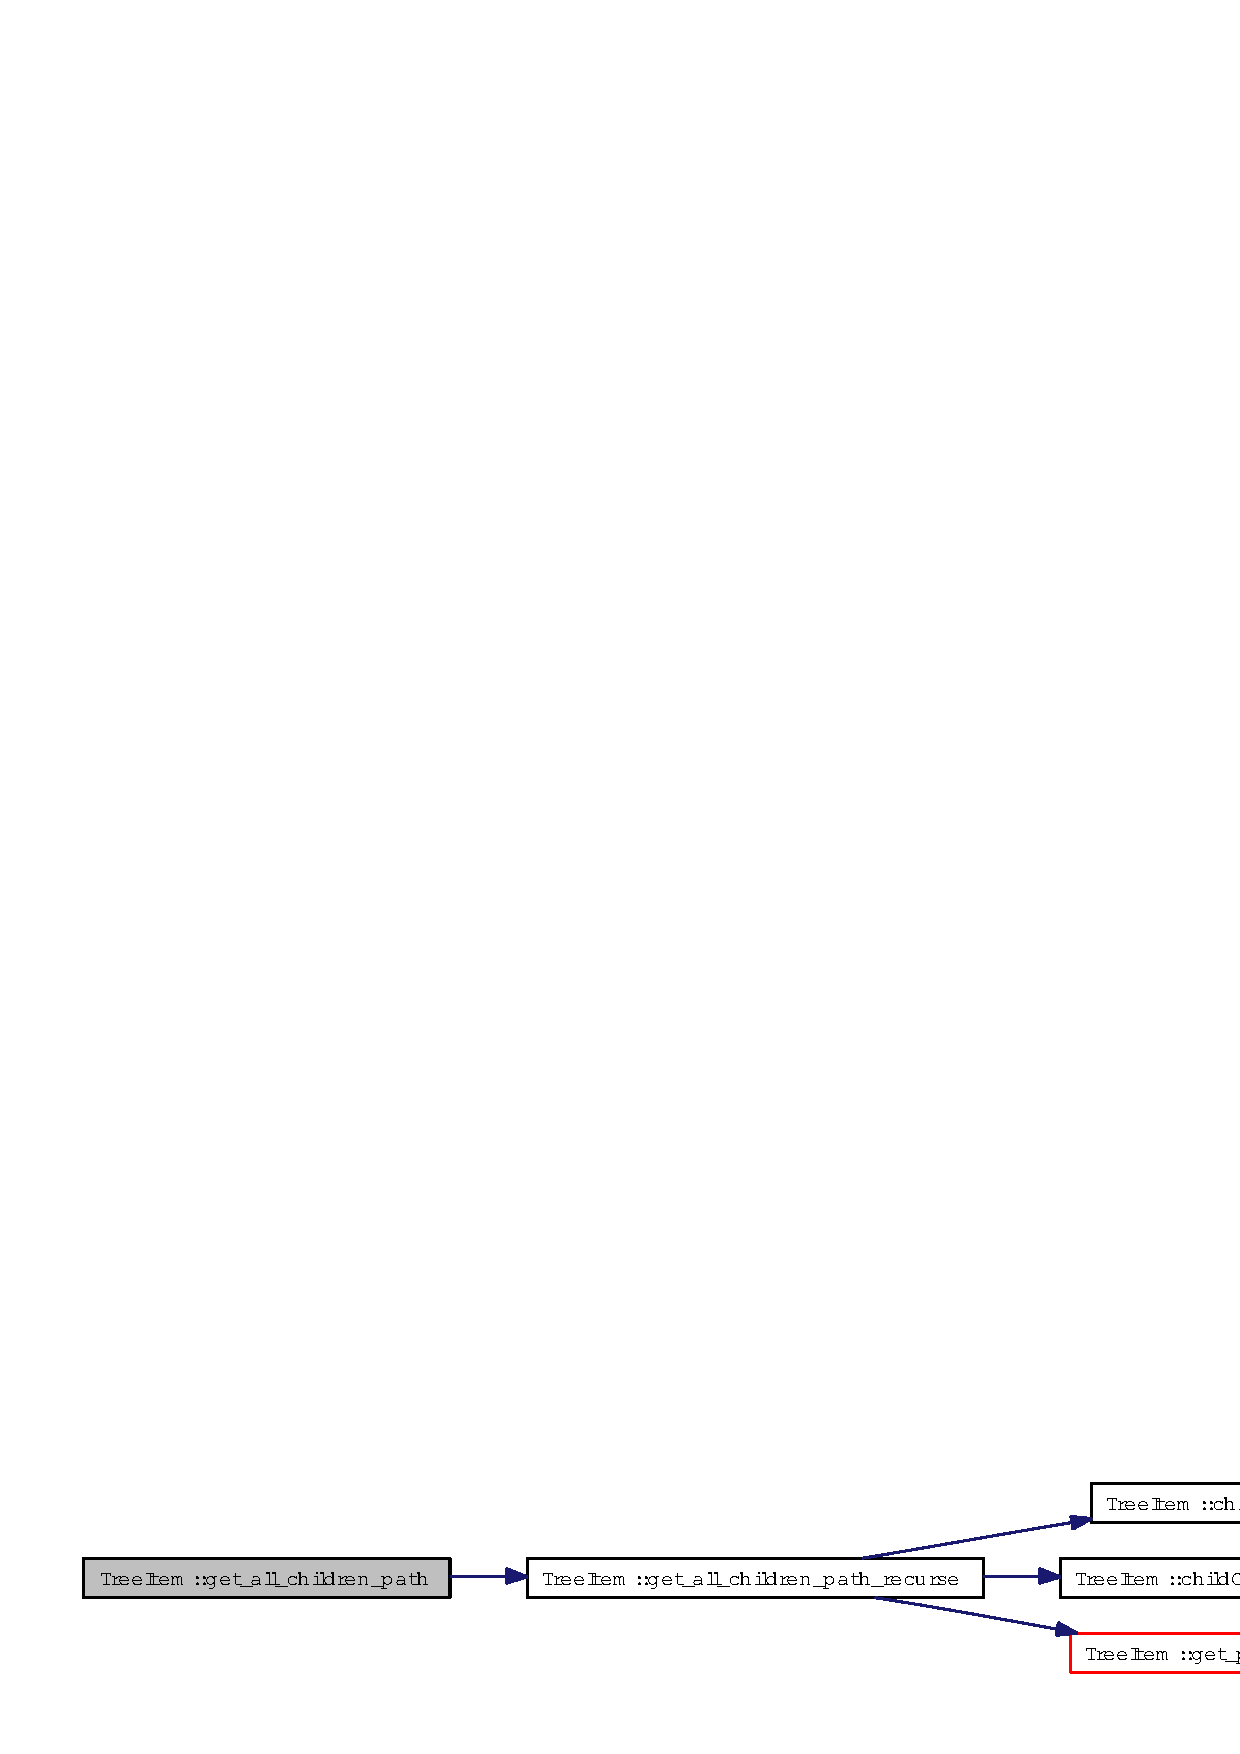
\includegraphics[width=318pt]{classTreeItem_cd5987be73e4cd3a16003b6bad3f1e67_cgraph}
\end{center}
\end{figure}
\index{TreeItem@{Tree\-Item}!recordtable_init@{recordtable\_\-init}}
\index{recordtable_init@{recordtable\_\-init}!TreeItem@{Tree\-Item}}
\subsubsection{\setlength{\rightskip}{0pt plus 5cm}void Tree\-Item::recordtable\_\-init (QDom\-Element {\em dommodel})}\label{classTreeItem_9f44b2a7b41bc5f791cc25732e41cae6}




Definition at line 285 of file treeitem.cpp.

References recordtabledata::init(), and rtable.

Referenced by knowtreemodel::parsenodeelement().

Here is the call graph for this function:\begin{figure}[H]
\begin{center}
\leavevmode
\includegraphics[width=300pt]{classTreeItem_9f44b2a7b41bc5f791cc25732e41cae6_cgraph}
\end{center}
\end{figure}


Here is the caller graph for this function:\begin{figure}[H]
\begin{center}
\leavevmode
\includegraphics[width=324pt]{classTreeItem_9f44b2a7b41bc5f791cc25732e41cae6_icgraph}
\end{center}
\end{figure}
\index{TreeItem@{Tree\-Item}!recordtable_getrowcount@{recordtable\_\-getrowcount}}
\index{recordtable_getrowcount@{recordtable\_\-getrowcount}!TreeItem@{Tree\-Item}}
\subsubsection{\setlength{\rightskip}{0pt plus 5cm}int Tree\-Item::recordtable\_\-getrowcount (void)}\label{classTreeItem_f736d45c591daa6e3a00da91a61c593b}




Definition at line 291 of file treeitem.cpp.

References rtable, and recordtabledata::size().

Referenced by Tree\-Model::data(), data(), findscreen::find\_\-recurse(), and knowtreemodel::parsetreetodom().

Here is the call graph for this function:\begin{figure}[H]
\begin{center}
\leavevmode
\includegraphics[width=200pt]{classTreeItem_f736d45c591daa6e3a00da91a61c593b_cgraph}
\end{center}
\end{figure}


Here is the caller graph for this function:\begin{figure}[H]
\begin{center}
\leavevmode
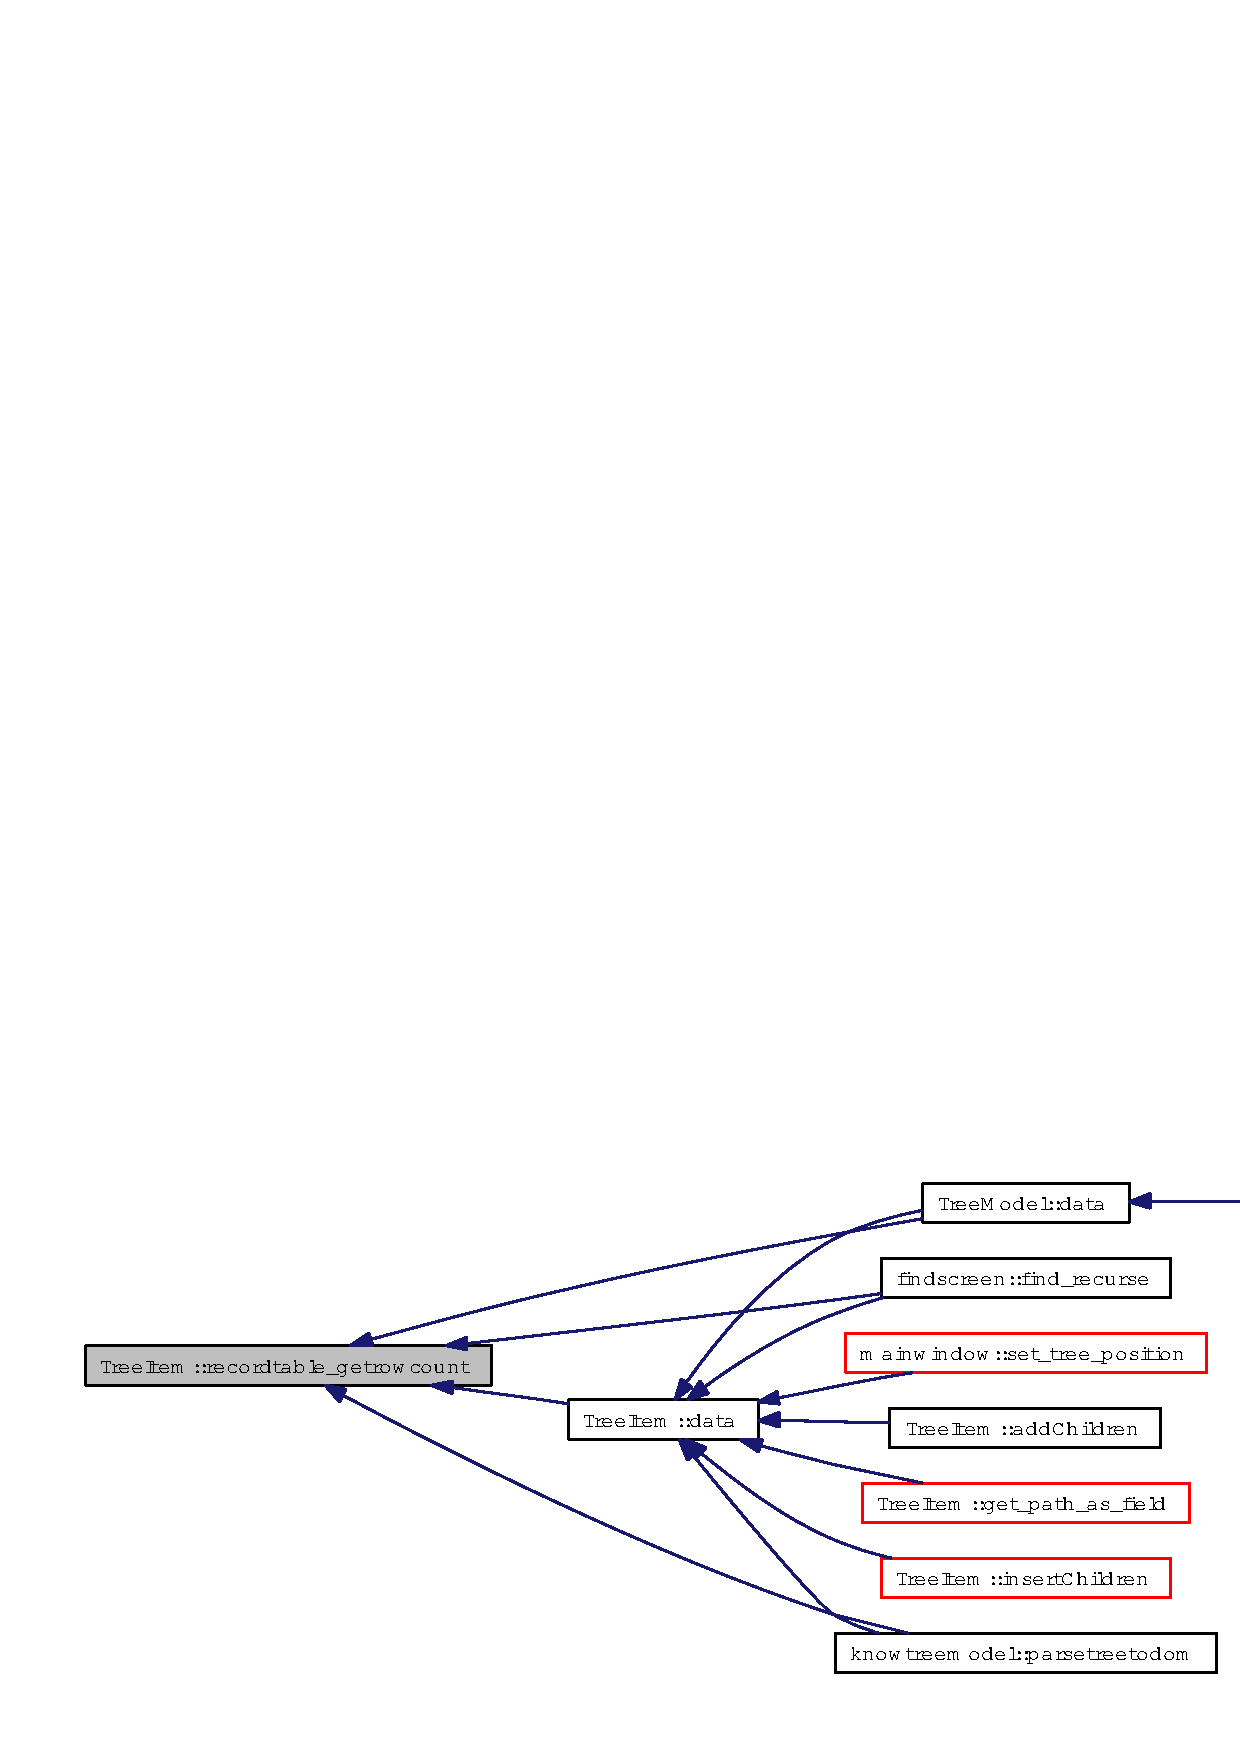
\includegraphics[width=370pt]{classTreeItem_f736d45c591daa6e3a00da91a61c593b_icgraph}
\end{center}
\end{figure}
\index{TreeItem@{Tree\-Item}!recordtable_clear@{recordtable\_\-clear}}
\index{recordtable_clear@{recordtable\_\-clear}!TreeItem@{Tree\-Item}}
\subsubsection{\setlength{\rightskip}{0pt plus 5cm}void Tree\-Item::recordtable\_\-clear (void)}\label{classTreeItem_409019fbc34a4e4bb315904d72ba44ce}




Definition at line 303 of file treeitem.cpp.

References recordtabledata::clear(), and rtable.

Referenced by $\sim$Tree\-Item().

Here is the call graph for this function:\begin{figure}[H]
\begin{center}
\leavevmode
\includegraphics[width=395pt]{classTreeItem_409019fbc34a4e4bb315904d72ba44ce_cgraph}
\end{center}
\end{figure}


Here is the caller graph for this function:\begin{figure}[H]
\begin{center}
\leavevmode
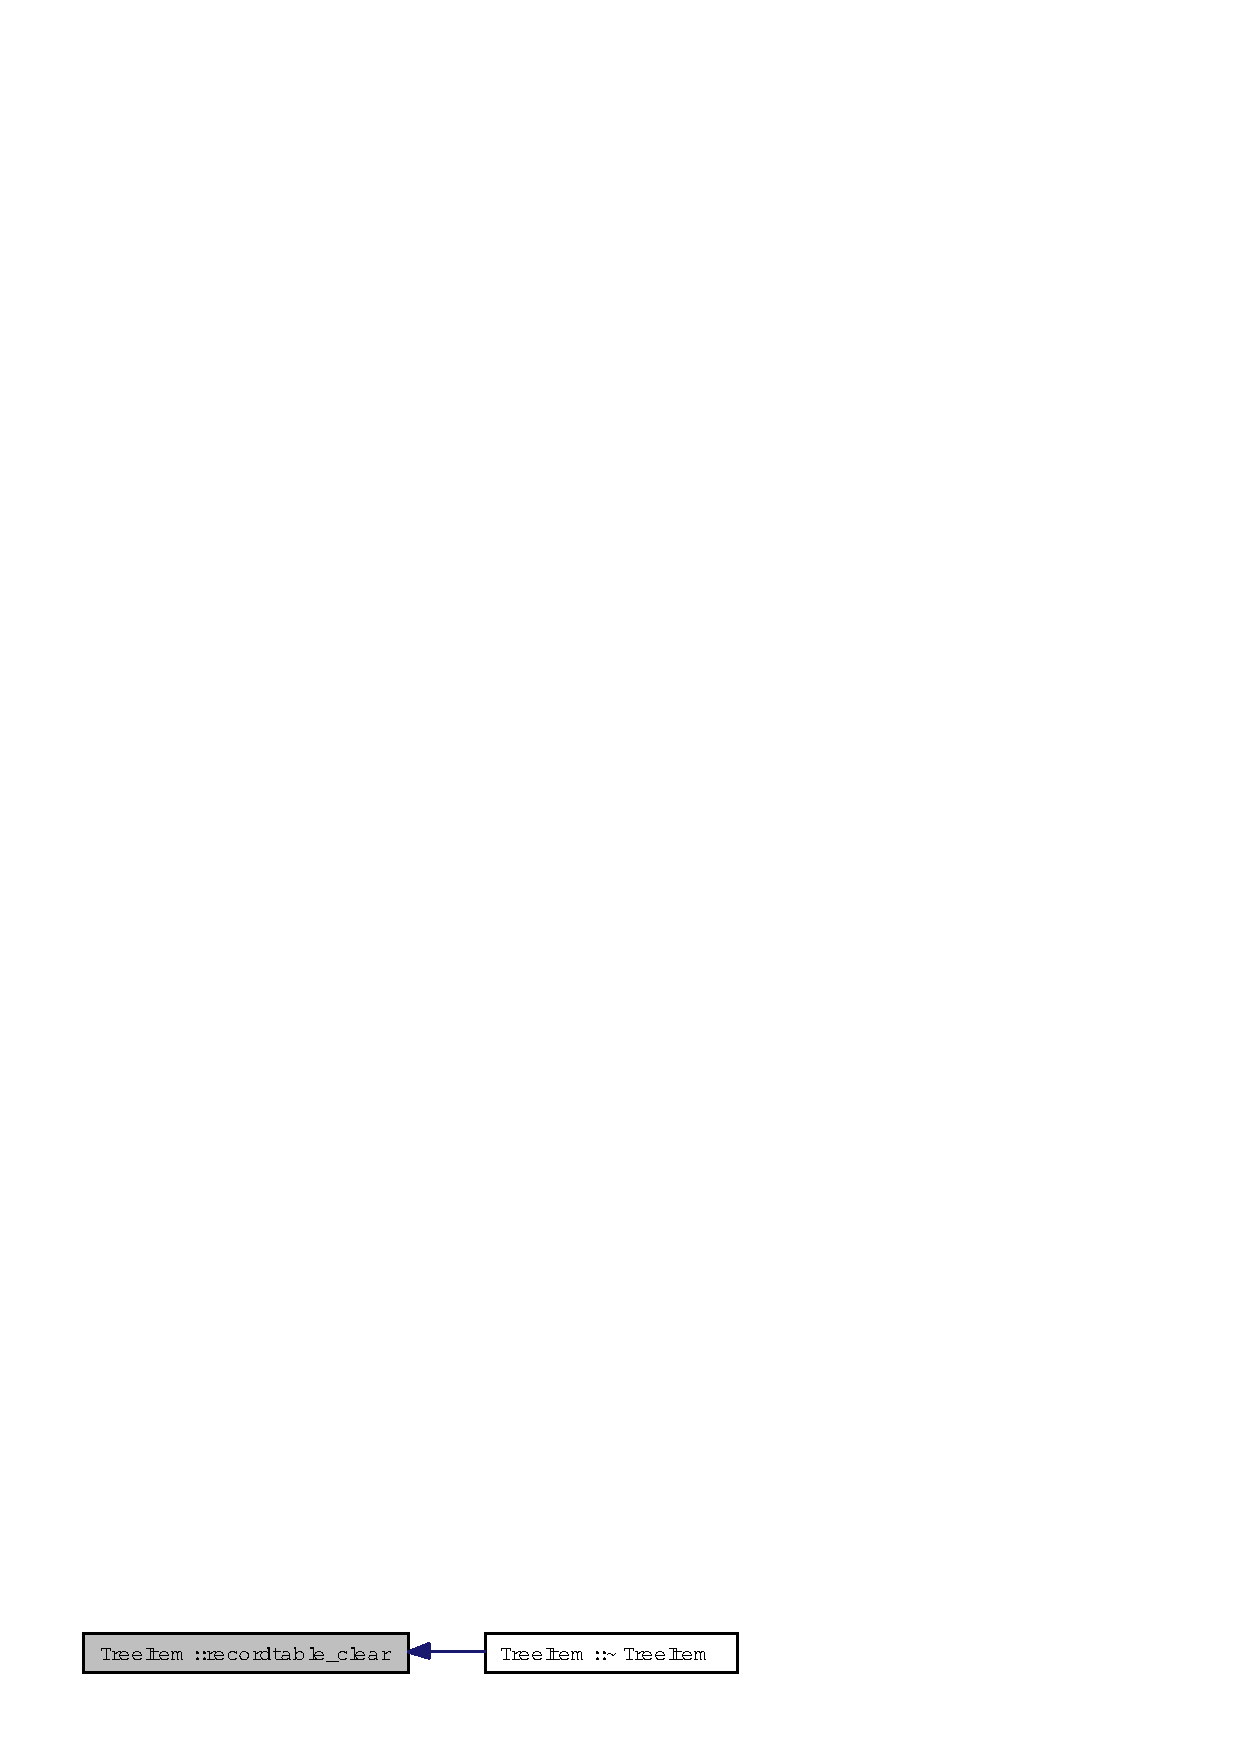
\includegraphics[width=179pt]{classTreeItem_409019fbc34a4e4bb315904d72ba44ce_icgraph}
\end{center}
\end{figure}
\index{TreeItem@{Tree\-Item}!recordtable_export_data_to_dom@{recordtable\_\-export\_\-data\_\-to\_\-dom}}
\index{recordtable_export_data_to_dom@{recordtable\_\-export\_\-data\_\-to\_\-dom}!TreeItem@{Tree\-Item}}
\subsubsection{\setlength{\rightskip}{0pt plus 5cm}QDom\-Document Tree\-Item::recordtable\_\-export\_\-data\_\-to\_\-dom (void)}\label{classTreeItem_0881f776f987c732545d57a4553ed405}




Definition at line 297 of file treeitem.cpp.

References recordtabledata::export\_\-data\_\-to\_\-dom(), and rtable.

Referenced by knowtreemodel::parsetreetodom().

Here is the call graph for this function:\begin{figure}[H]
\begin{center}
\leavevmode
\includegraphics[width=261pt]{classTreeItem_0881f776f987c732545d57a4553ed405_cgraph}
\end{center}
\end{figure}


Here is the caller graph for this function:\begin{figure}[H]
\begin{center}
\leavevmode
\includegraphics[width=394pt]{classTreeItem_0881f776f987c732545d57a4553ed405_icgraph}
\end{center}
\end{figure}
\index{TreeItem@{Tree\-Item}!recordtable_gettabledata@{recordtable\_\-gettabledata}}
\index{recordtable_gettabledata@{recordtable\_\-gettabledata}!TreeItem@{Tree\-Item}}
\subsubsection{\setlength{\rightskip}{0pt plus 5cm}{\bf recordtabledata} $\ast$ Tree\-Item::recordtable\_\-gettabledata (void)}\label{classTreeItem_8f23227037841048efa95d2e22d0c2d7}




Definition at line 308 of file treeitem.cpp.

References rtable.

Referenced by findscreen::find\_\-recurse(), and treescreen::on\_\-knowtree\_\-clicked().

Here is the caller graph for this function:\begin{figure}[H]
\begin{center}
\leavevmode
\includegraphics[width=288pt]{classTreeItem_8f23227037841048efa95d2e22d0c2d7_icgraph}
\end{center}
\end{figure}
\index{TreeItem@{Tree\-Item}!removeChildrenLink@{removeChildrenLink}}
\index{removeChildrenLink@{removeChildrenLink}!TreeItem@{Tree\-Item}}
\subsubsection{\setlength{\rightskip}{0pt plus 5cm}bool Tree\-Item::remove\-Children\-Link (int {\em position}, int {\em count})\hspace{0.3cm}{\tt  [private]}}\label{classTreeItem_8f1bcb3b23412364f198e4782058a0e4}




Definition at line 169 of file treeitem.cpp.

References child\-Items.\index{TreeItem@{Tree\-Item}!get_all_children_path_recurse@{get\_\-all\_\-children\_\-path\_\-recurse}}
\index{get_all_children_path_recurse@{get\_\-all\_\-children\_\-path\_\-recurse}!TreeItem@{Tree\-Item}}
\subsubsection{\setlength{\rightskip}{0pt plus 5cm}QList$<$ QString\-List $>$ Tree\-Item::get\_\-all\_\-children\_\-path\_\-recurse ({\bf Tree\-Item} $\ast$ {\em item}, int {\em mode})\hspace{0.3cm}{\tt  [private]}}\label{classTreeItem_35eb0e9477ec77668faf4040617df48d}




Definition at line 262 of file treeitem.cpp.

References child(), child\-Count(), and get\_\-path().

Referenced by get\_\-all\_\-children\_\-path().

Here is the call graph for this function:\begin{figure}[H]
\begin{center}
\leavevmode
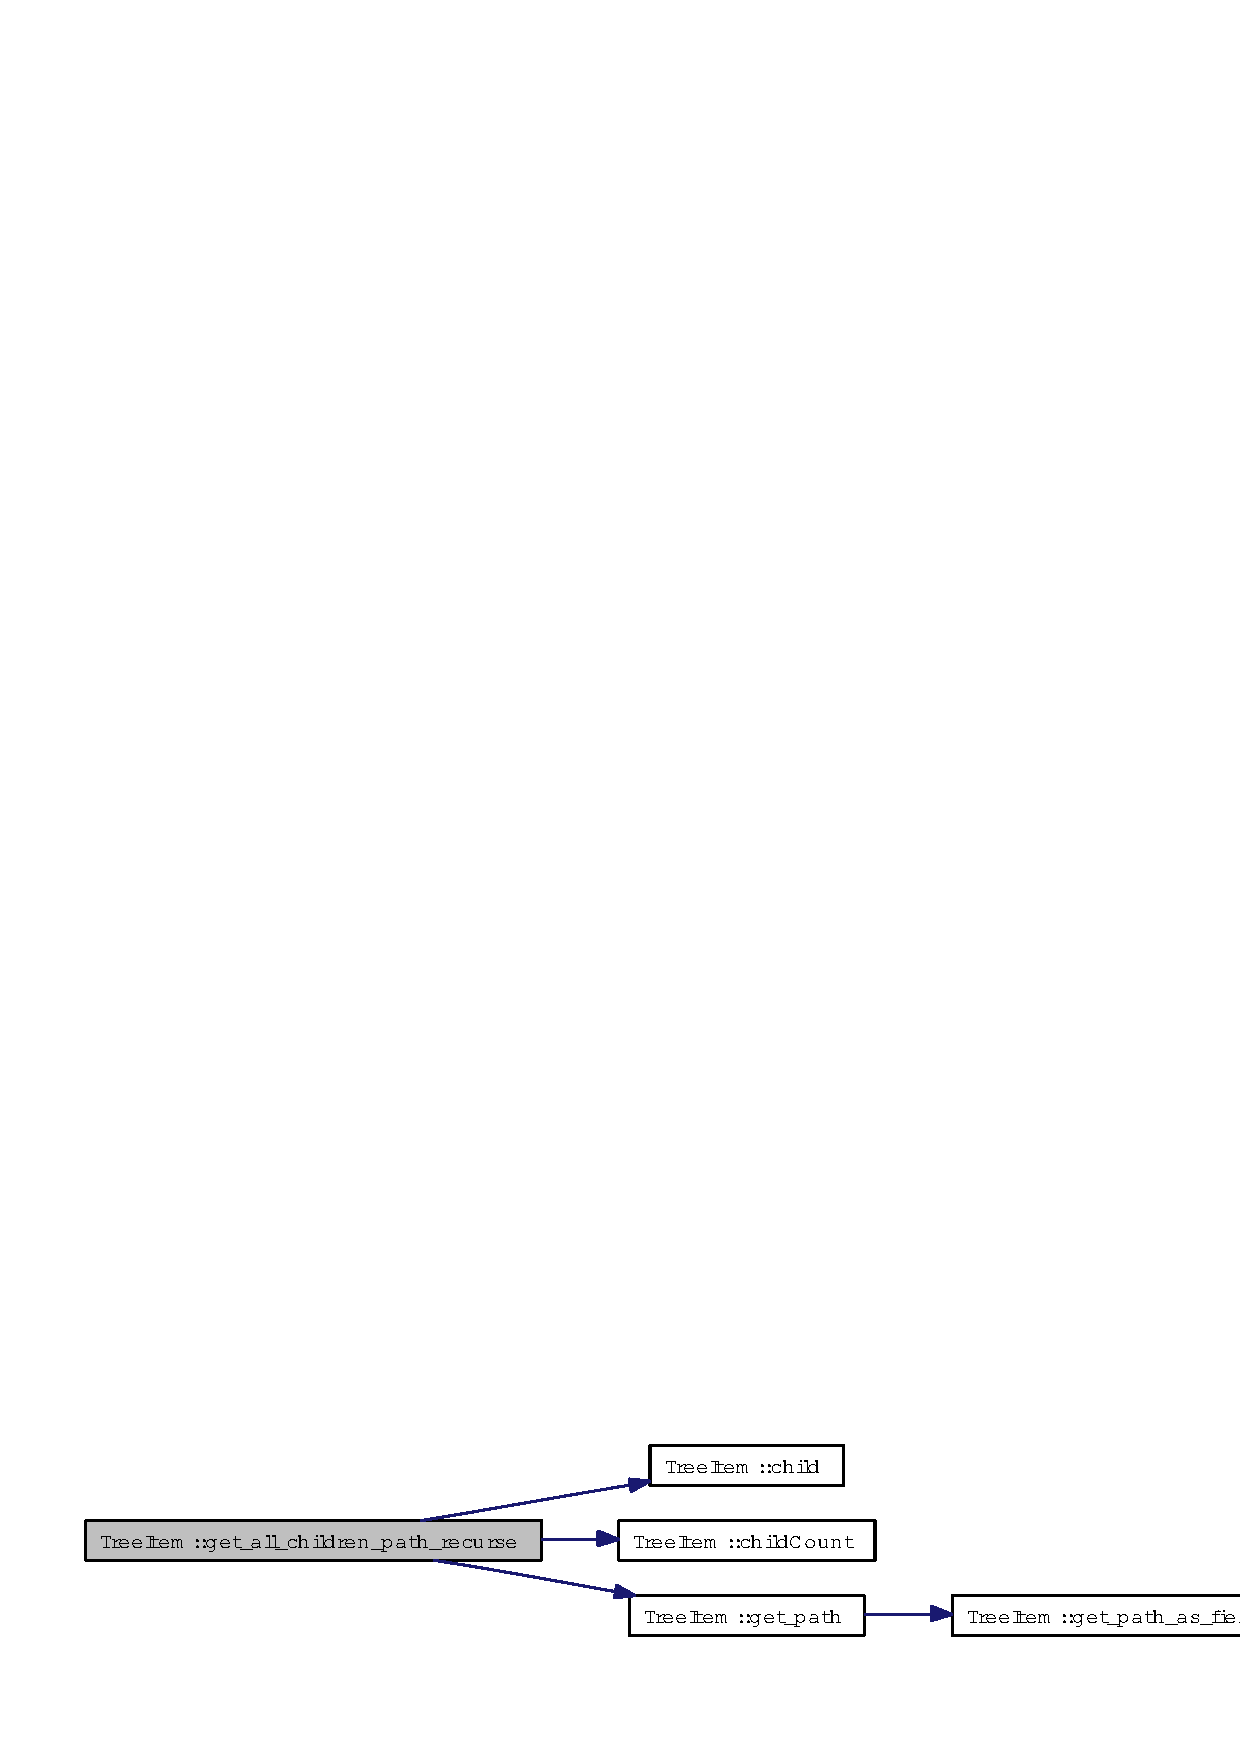
\includegraphics[width=378pt]{classTreeItem_35eb0e9477ec77668faf4040617df48d_cgraph}
\end{center}
\end{figure}


Here is the caller graph for this function:\begin{figure}[H]
\begin{center}
\leavevmode
\includegraphics[width=238pt]{classTreeItem_35eb0e9477ec77668faf4040617df48d_icgraph}
\end{center}
\end{figure}
\index{TreeItem@{Tree\-Item}!get_path_as_field@{get\_\-path\_\-as\_\-field}}
\index{get_path_as_field@{get\_\-path\_\-as\_\-field}!TreeItem@{Tree\-Item}}
\subsubsection{\setlength{\rightskip}{0pt plus 5cm}QString\-List Tree\-Item::get\_\-path\_\-as\_\-field (QString {\em field})\hspace{0.3cm}{\tt  [private]}}\label{classTreeItem_a55f28f0c0a558f914759a6c8ebb28b9}




Definition at line 225 of file treeitem.cpp.

References data(), and parent().

Referenced by get\_\-path(), and get\_\-path\_\-as\_\-name().

Here is the call graph for this function:\begin{figure}[H]
\begin{center}
\leavevmode
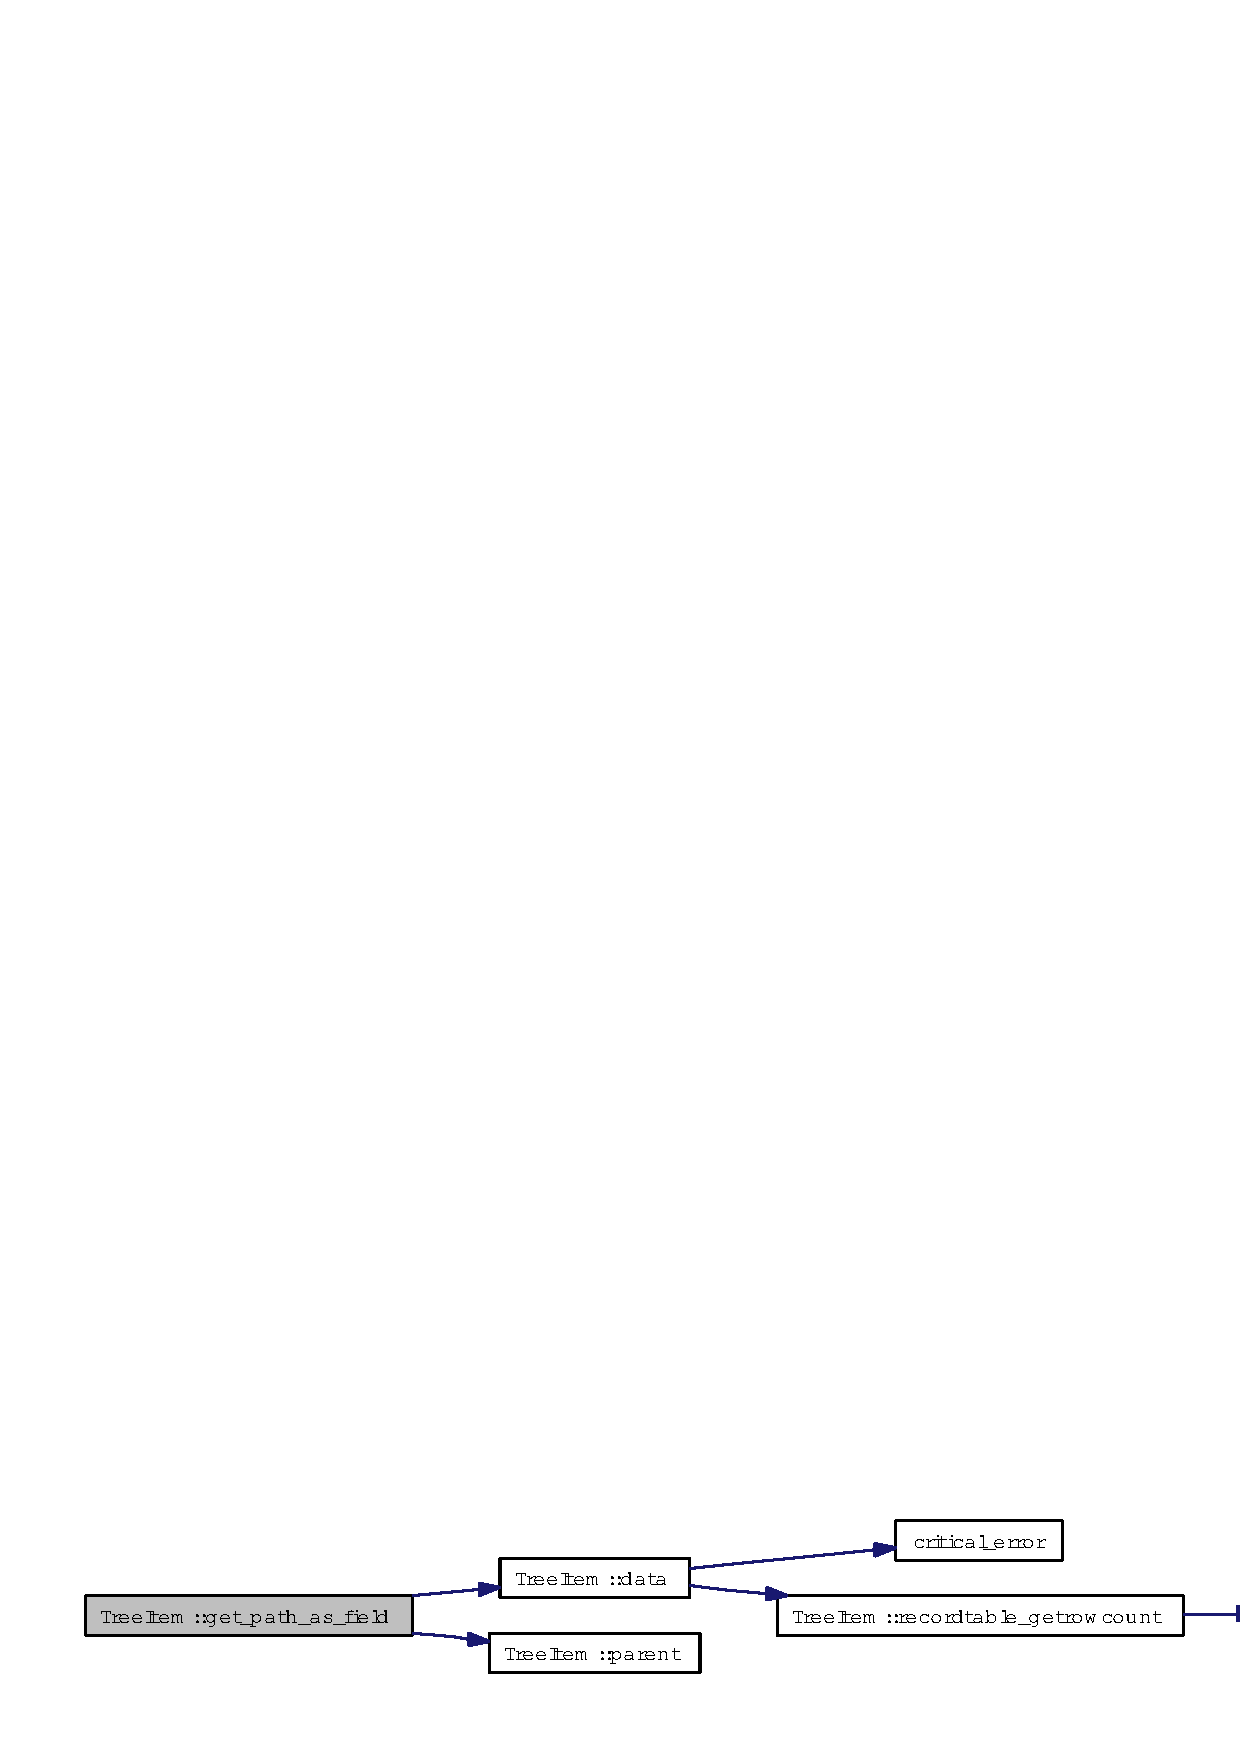
\includegraphics[width=366pt]{classTreeItem_a55f28f0c0a558f914759a6c8ebb28b9_cgraph}
\end{center}
\end{figure}


Here is the caller graph for this function:\begin{figure}[H]
\begin{center}
\leavevmode
\includegraphics[width=329pt]{classTreeItem_a55f28f0c0a558f914759a6c8ebb28b9_icgraph}
\end{center}
\end{figure}


\subsection{Member Data Documentation}
\index{TreeItem@{Tree\-Item}!childItems@{childItems}}
\index{childItems@{childItems}!TreeItem@{Tree\-Item}}
\subsubsection{\setlength{\rightskip}{0pt plus 5cm}QList$<${\bf Tree\-Item}$\ast$$>$ {\bf Tree\-Item::child\-Items}\hspace{0.3cm}{\tt  [private]}}\label{classTreeItem_7ea3d75732252074ae15587693b4fa01}




Definition at line 87 of file treeitem.h.

Referenced by add\-Children(), child(), child\-Count(), child\-Number(), insert\-Children(), move\_\-dn(), move\_\-up(), remove\-Children(), remove\-Children\-Link(), and $\sim$Tree\-Item().\index{TreeItem@{Tree\-Item}!parentItem@{parentItem}}
\index{parentItem@{parentItem}!TreeItem@{Tree\-Item}}
\subsubsection{\setlength{\rightskip}{0pt plus 5cm}{\bf Tree\-Item}$\ast$ {\bf Tree\-Item::parent\-Item}\hspace{0.3cm}{\tt  [private]}}\label{classTreeItem_24d1acb93b04dbf0f67036263d87b8af}




Definition at line 88 of file treeitem.h.

Referenced by child\-Number(), move\_\-dn(), move\_\-up(), parent(), and Tree\-Item().\index{TreeItem@{Tree\-Item}!fieldtable@{fieldtable}}
\index{fieldtable@{fieldtable}!TreeItem@{Tree\-Item}}
\subsubsection{\setlength{\rightskip}{0pt plus 5cm}QMap$<$QString, QString$>$ {\bf Tree\-Item::fieldtable}\hspace{0.3cm}{\tt  [private]}}\label{classTreeItem_373cdc232a457da1761e4e7136d1586a}




Definition at line 91 of file treeitem.h.

Referenced by data(), field\-Count(), set\-Data(), and Tree\-Item().\index{TreeItem@{Tree\-Item}!rtable@{rtable}}
\index{rtable@{rtable}!TreeItem@{Tree\-Item}}
\subsubsection{\setlength{\rightskip}{0pt plus 5cm}{\bf recordtabledata} {\bf Tree\-Item::rtable}\hspace{0.3cm}{\tt  [private]}}\label{classTreeItem_cf2a253a2d4fc5f803b21d7bce0582ee}




Definition at line 94 of file treeitem.h.

Referenced by recordtable\_\-clear(), recordtable\_\-export\_\-data\_\-to\_\-dom(), recordtable\_\-getrowcount(), recordtable\_\-gettabledata(), and recordtable\_\-init().

The documentation for this class was generated from the following files:\begin{CompactItemize}
\item 
{\bf treeitem.h}\item 
{\bf treeitem.cpp}\end{CompactItemize}
